\documentclass[oneside,final,14pt,a4paper]{extreport}

\usepackage{tempora} % Times New Roman alike font  

\usepackage{tabularx}

\usepackage{vmargin}
\setpapersize{A4}
\setmarginsrb{2.5cm}{2.2cm}{2.2cm}{2.2cm}{0pt}{10mm}{0pt}{13mm}
\usepackage{setspace}
\setstretch{1.5}
\usepackage{indentfirst}
\parindent=1.25cm

%%%%% ADDED TO SUPPORT TT BOLD FACES %%%%
\DeclareFontShape{OT1}{cmtt}{bx}{n}{<5><6><7><8><9><10><10.95><12><14.4><17.28><20.74><24.88>cmttb10}{}
\renewcommand{\ttdefault}{pcr}
%%%%% END %%%%%%%%%%%%%%%%%%%%%%%%%%%%%%% 

\usepackage{atbegshi,picture}
\usepackage[T1,T2A]{fontenc}
\usepackage[utf8]{inputenc}

\usepackage[english]{babel}
\usepackage[backend=biber,style=ieee,autocite=inline]{biblatex}
\bibliography{ref.bib}
\DefineBibliographyStrings{english}{%
  bibliography = {References},}
\usepackage{blindtext}

\usepackage{pdfpages}
\newenvironment{bottompar}{\par\vspace*{\fill}}{\clearpage}
\usepackage{amsmath,amsfonts}
\usepackage{url}
\usepackage{amsthm}
\newtheorem{theorem}{Theorem}
\newtheorem{corollary}{Corollary}
\newtheorem{lemma}{Lemma}
\newtheorem{proposition}{Proposition}
\theoremstyle{definition}
\newtheorem{definition}{Definition}
\theoremstyle{remark}
\newtheorem*{remark}{Remark}
\theoremstyle{remark}
\newtheorem*{example}{Example}

\usepackage{float}
\usepackage{graphicx}
\graphicspath{{figs/}} %path to images
\usepackage{array}
\usepackage{multirow,array}
\usepackage{caption}
\usepackage{subcaption}
\usepackage{hyperref}
\hypersetup{colorlinks=true, linkcolor=black, citecolor=black}
\usepackage{paralist}
\usepackage{listings}
\usepackage{zed-csp}
\usepackage{fancyhdr}
\usepackage{csquotes}
\usepackage{color}
% \usepackage{anyfontsize}
% \usepackage{mathptmx}
% \usepackage{t1enc}

\usepackage{chngcntr}
\usepackage{upgreek} 
\usepackage{bm}
\usepackage{hyperref}
\usepackage{booktabs}
\usepackage{multirow}
\usepackage{longtable}
\usepackage[font=singlespacing, labelfont=bf]{caption}
%Hints
\newcommand\pic[1]{(Fig. \ref{#1})} %Ref on figure
\newcommand\tab[1]{(Tab. \ref{#1})} %Ref on table

\setlength{\headheight}{32.0976pt}
\usepackage{enumitem}
\newlist{inlinelist}{enumerate*}{1}
\setlist*[inlinelist,1]{%
  label=(\arabic*),
}

% \setcounter{secnumdepth}{4}
\captionsetup[table]{labelfont={normalfont}, name={TABLE}, labelsep={newline}}
\setlength{\parindent}{2em} 
\DeclareCaptionLabelSeparator{figSep}{.\quad}
\captionsetup[figure]{labelfont={normalfont}, name={Fig.}, labelsep=period}
\counterwithin{figure}{chapter}

% \usepackage{titlesec}
% \titleformat{\section}[hang]{\fontsize{20}{24}\selectfont\filcenter}{\Roman{section}}{1em}{}
% \titleformat{\subsection}[hang]{\itshape}{\Alph{subsection}.}{1em}{}[]
% \titleformat{\subsubsection}[runin]{\itshape}{\arabic{subsubsection})}{1em}{}[$:$]
% \titlespacing{\subsubsection}{1em}{1em}{1em}
% \titleformat{\paragraph}[runin]{\itshape}{\alph{paragraph})}{1em}{}[$:$\quad]
% \titlespacing{\paragraph}{2em}{1em}{1em}

\usepackage{placeins} % for \FloatBarrier

\pagestyle{fancyplain}

% remember section title
\renewcommand{\chaptermark}[1]%
	{\markboth{\chaptername~\thechapter~--~#1}{}}

% subsection number and title
\renewcommand{\sectionmark}[1]%
	{\markright{\thesection\ #1}}

\rhead[\fancyplain{}{\bf\leftmark}]%
      {\fancyplain{}{\bf\thepage}}
\lhead[\fancyplain{}{\bf\thepage}]%
      {\fancyplain{}{\bf\rightmark}}
\cfoot{} %bfseries


\newcommand{\dedication}[1]
   {\thispagestyle{empty}
     
   \begin{flushleft}\raggedleft #1\end{flushleft}
}


\begin{document}

\tableofcontents
\listoftables
\listoffigures
\newpage


\begin{abstract}
In this paper, I study the existing metrics for evaluating text-to-image generative models. I divide the current metrics into distance metrics and score metrics. I conduct various experiments in order to deduce the best metric and evaluate metrics in such a way that one metric is considered better than another if it correlates better with human judgement. The main contributions are the derivation of the best distance metric is FD\_DINOv2, the derivation of the best score metrics is ImageReward and the creation of it is own metric COS\_DINOv2, which differs from both distance metrics and score metrics. FD\_DINOv2 is a metric that uses DINOv2 to get embeddings from images and fréchet distance to calculate the distance between two distributions - embeddings of real and generated images. ImageReward is an improved version of the CLIPScore metric. COS\_DINOv2 is a metric that uses DINOv2 to get embeddings from images and for each pair of embeddings calculate a score that shows how similarity of the embeddings of the real and generated images, respectively showing how similar the real and generated images are.
\end{abstract}
\setcounter{page}{10}
% set manually the number, from which Chapter 1 starts!
% Why do we put 7 in this case?
% Title page - page 1
% Contents - page 2, page 3
% List of tables - page 4
% List of figures - page 5
% Abstract - page 6
% Chapter 1 - page 7
% In your thesis the counter number can be different, please count carefully and insert the corresponding number.

\chapter{Introduction}
\label{chap:intro}
\chaptermark{Optional running chapter heading}

Text-to-image models have been actively developed recently.  Recent models \cite{Imagen}\cite{PixArt}\cite{Latent_Diffusion}\cite{Casceded_Diffusion}\cite{Stable_Duffusion} have made great strides in creating realistic images that exactly follow the textual description. Researchers have constructed a set of metrics designed to assess the quality and effectiveness of these models. Metrics should evaluate the individual characteristics of a set of generated pictures and their description(prompts) such as defective, aesthetically pleasing, fidelity, text-to-image, diversity, and rarity. The ultimate objective is to ensure that the metric's evaluation of the generative model is reflective of human evaluative standards.

Unfortunately, an estimate of the generated images made with the current most commonly used metrics may not match the human judgement. There's also the problem that there are no metrics that separately assess individual characteristics.

At the moment, two of the more commonly used metrics for generative models are CLIPScore \cite{CLIPScore} and Frechet Inception Distance (FID) \cite{FID}. The idea behind the CLIPScore metric is to use the CLIP(Contrastive Language-Image Pretraining) \cite{CLIP} model to create latent vector representation(embedding) for image and text and count their consine simmularity to estimate the text to image alignment. To count CLIPScore you only need prompts, a text description of what to generate. The idea of FID is to create embeddings for the generated images and for the real images and compare them using Fréchet Distance(FD). FID indicates how well the image generation model generates images similar to real images. To estimate the calculation of the FID metric I need generated images and real images to which the generated images should resemble.

% There are already methods to improve FID and CLIPScore. In FID, researchers change the way the distance between distributions is calculated, as well as the method of embedding. In CLIPScore, researchers change the CLIP architecture to an improved one, such as BLIP \cite{BLIP}, and do some fine-tune on special datasets.

Current metrics can be divided into two types: metrics that count the distance between the embeddings of real images and the generated ones, and metrics that give the pair of the generated image and the prompt some score. In what follows, I will refer to the first type of metrics as distance metrics and the second as score metrics.

At the moment there is no complete comparison of all metrics to determine the best one. There is also no clear distinction between what a metric measures: defective, aesthetically pleasing, fidelity, text-to-image, diversity, or rarity. Some metrics show unrealistic results, such as FID. Almost all metrics do not correlate with human judgement or correlate very weakly.

 The contributions of this thesis are as follows:
 \begin{itemize}
  \item Analysing existing metrics, validating and comparing them on the same data, using the same image generation model. Measuring the correlation of existing metrics with human judgement.
  \item Running experiments with current metrics to try to improve them. For example, changing the model for embeddings and the method of measuring similarity of distributions for real and generated images in distance metrics, improving the CLIP model in score metrics.
  \item Writing my own metric which based on idea of distance metric, but which requires not only real images but prompts which relates to real images. Idea is to use information that real image and generated image realise the same prompt.
\end{itemize}






\chapter{Literature Review}
\label{chap:lr}
\chaptermark{Second Chapter Heading}

\section{Frechet Inception Distance}
The Fréchet Inception Distance(FID) is the distance metric. Idea behind each distance metric is to extract features from two datasets of pictures and then calculate distance between two datasets. Resulting scalar will be result of the metric. Extracted features may also be called embeddings: it is a vector of low dimensionality with respect to the dimensionality of the image. For clarity, I have made a diagram of the FID metric as a example of distance metric.
\begin{figure}[hbt]
\centering
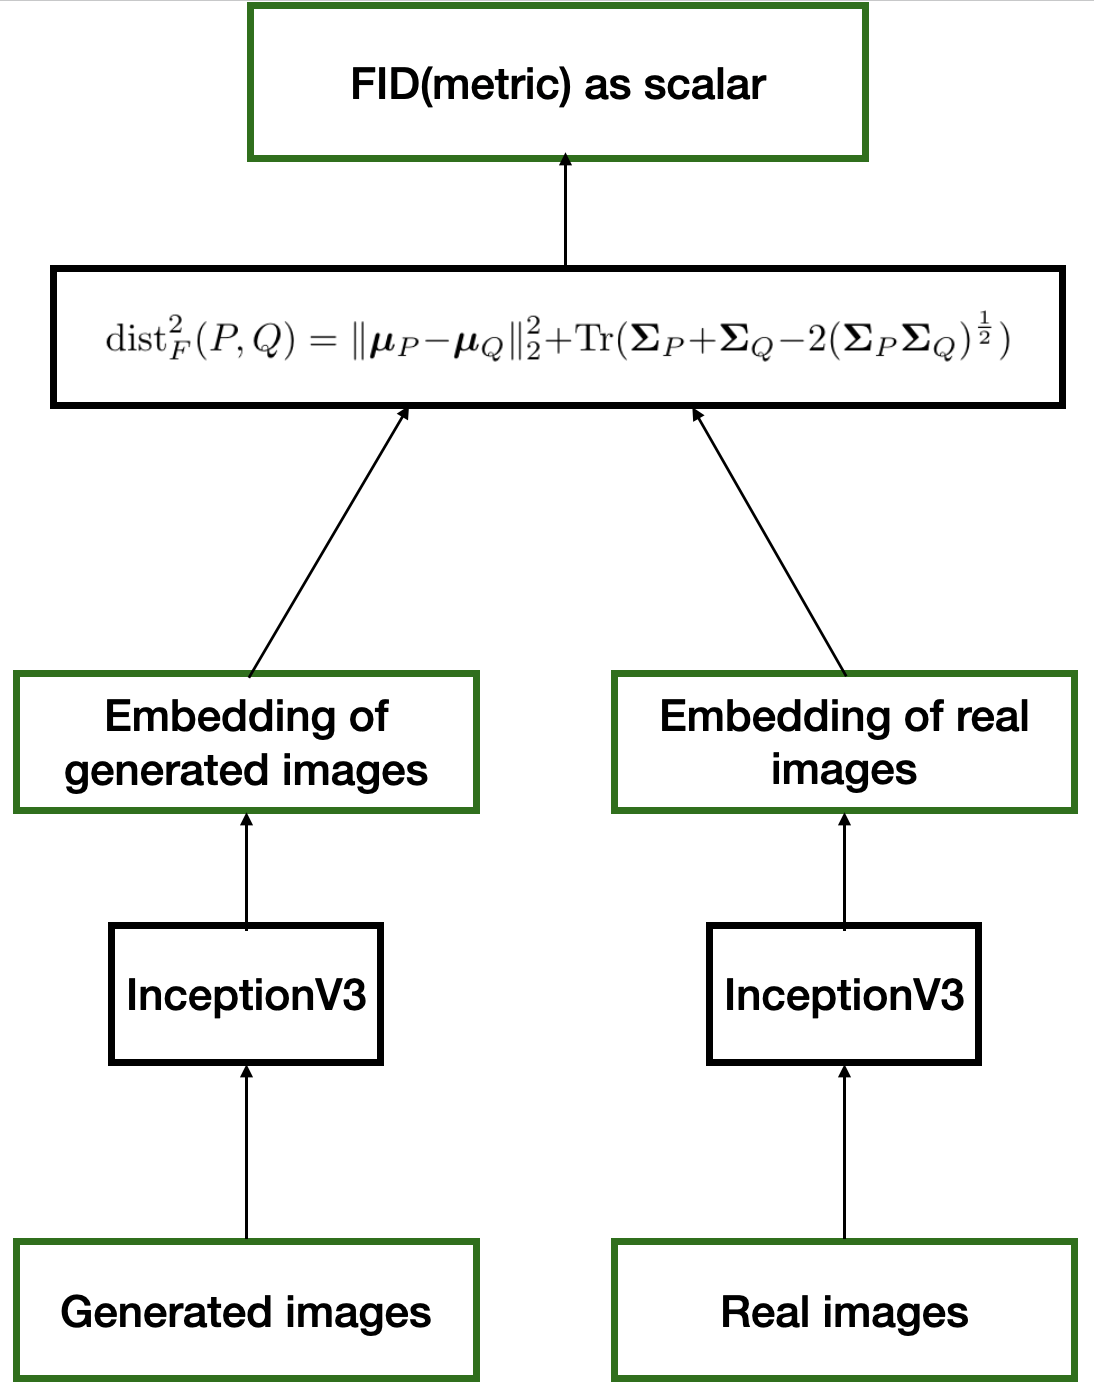
\includegraphics[width=10cm, height=12cm]{figs/fid_diagram.png}
\caption{The diagram of Fréchet Inception Distance(FID). Where $\mu_P$ , $\mu_Q$ are the means and $\Sigma_P$ , $\Sigma_Q$ are the covariances of the two multivariate normal distributions $P$ and $Q$}
\label{fig:FID_diagram}
\end{figure}
As show in the Figure~\ref{fig:FID_diagram}, fréchet inception distance (FID) metric uses the convolutional network InceptionV3 to compute image embeddings and fréchet distance for calculating distance between two datasets of embeddings.

The formula for calculating the Fréchet Distance taken from \cite{FD}:
\begin{equation}
dist^2_F(P,Q)=inf_{\gamma\in \Gamma(P,Q)}E_{(x,y)\gamma}\|x-y\|^2
\end{equation}
According to the authors of the \cite{KD_CLIP}: "$\Gamma(P, Q)$ is the set of all couplings of $P$ and $Q$. This is also equivalent to the Wasserstein-2 distance on $\mathbb{R}^d$. In general, obtaining a closed-form solution for the Fréchet distance is difficult". However, the authors of \cite{FD} showed that a closed-form solution exists for multivariate normal distributions in the form:
\begin{equation}
dist^2_F(P,Q)=\|\mu_P-\mu_Q\|_2^2+Tr(\Sigma_P+\Sigma_Q-2(\Sigma_P\Sigma_Q^{1/2})
\end{equation}
where $\mu_P$ , $\mu_Q$ are the means and $\Sigma_P$ , $\Sigma_Q$ are the covariances of the two multivariate normal distributions $P$ and $Q$. Formula (2.2) is valid only when both $P$ and $Q$ are multivariate normal distributions \cite{FD}.
\section{FID disadvantages}
The articles highlight several major disadvantages of FID. First, Sadeep highlights: "inception’s poor representation of the rich and varied content generated by modern text-to-image models" \cite[p.1]{KD_CLIP}. Analysis and improvement of existing offline metrics for evaluating the quality of diffusion models for text to image generation. Inception model \cite{InceptionV3} convolutional network that was trained for the classification task on the ImageNet dataset. Today, there are new network architectures that can replace inception network. Recent research papers  \cite{KD_CLIP}\cite{FD_DINOv2}\cite{FID_Med} have presented a critical analysis of the use of InceptionV3 in the FID metric. Evaluation results from previous studies \cite{KD_CLIP} revealed that FID may not reflect a person's actual view and may even increase with more steps in diffusion generative networks, when it is quite obvious that with more steps the image becomes better. Among the alternatives proposed, models such as DINOv2 \cite{DINOv2}(Distilled and Noisy Self-supervised learning framework) and CLIP \cite{CLIP}(Contrastive Language-Image Pretraining). The new feature extractors are expected to improve the metrics evaluation process, leading to more robust estimates of generative models.

Second, FID is biased as noted in \cite{unbiasedFID}. Due to FID is biased one model may receive a higher score than another just because one has a smaller bias term.

Third, fréchet distance require to calculate the $d \times d$ covariance matrix where $d$ is embedding's dimensionality. Since embeddings of images are high-dimensional, calculating of matrix is time consuming.

Fourth, use closed-form solution of fréchet distance justified if assumption about normality of two distributions is right. The claim that embeddings occur in a normal distribution has not been proved. This point will be revealed in feature chapters.

\section{CLIPScore model}
The CLIPScore is score metric. Idea behind each score metric is to extract features(embeddings) from prompt and generated image and calculate simmularity between two embeddings. Resulting scalar will be result of the metric.
\subsection{CLIP model}
For all score metrics which I found as feature extractors for prompts and generated images was used CLIP architecture \cite{CLIP} which showed in Figure~\ref{fig:CLIP}:
\begin{figure}[hbt]
\centering
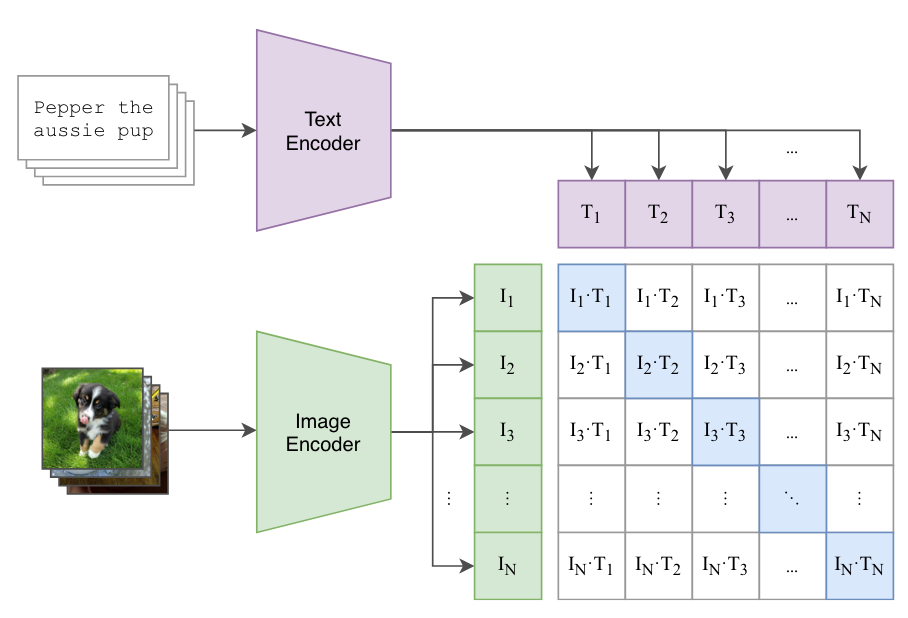
\includegraphics[width=12cm, height=8cm]{figs/clip.png}
\caption{Texts(prompts) and images encoded using Text Encoder and Image Encoder respectivly. Calculating cosine simularity for each pair of text and image from batch. CLIP architecture taken from \cite{CLIP}}
\label{fig:CLIP}
\end{figure}


The core idea behind CLIP is to align the image and text feature vectors in a high-dimensional space. Lets name the positive pair of image and text if we know that text associated to image and negative otherwise. Positive pairs of image and text should be close to each other in the feature space while negative pairs should be far apart. CLIP is trained on a large and diverse dataset collected from the internet, allowing it to learn from a broad range of visual styles, concepts, and natural language.


Once trained, CLIP can perform "zero-shot" learning, meaning it can correctly classify images into categories it has never seen during training, based only on textual descriptions of those categories. And also due to its training on a diverse internet-sourced dataset, CLIP generalizes well across different domains and types of images and descriptions.


To be clear I include pseudocode of CLIP training:
\begin{figure}[hbt]
\centering
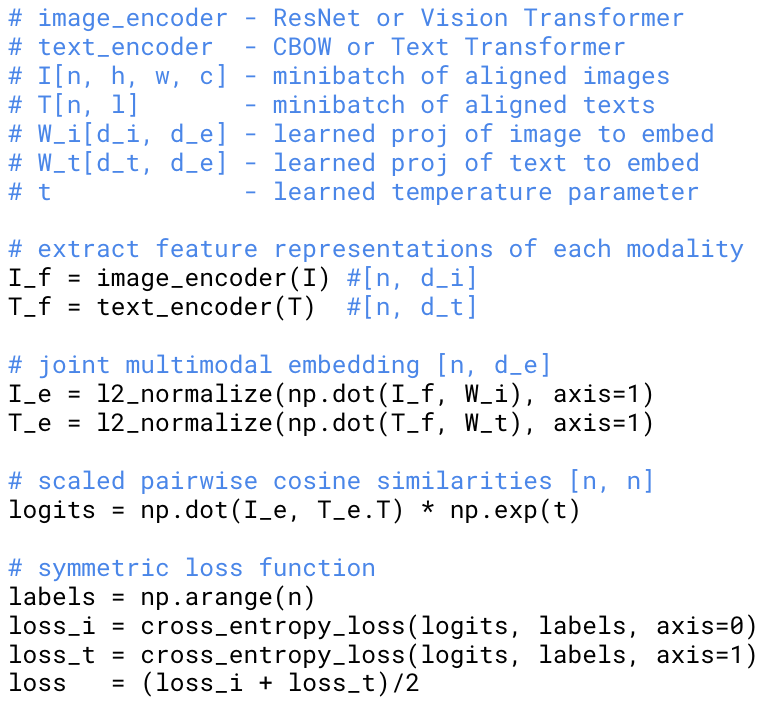
\includegraphics[width=12cm, height=10cm]{figs/clip_pseudocode.png}
\caption{Numpy-like pseudocode for the core of an implementation of CLIP. Taken from article\cite{CLIP}}
\label{fig:CLIP_pseudocode}
\end{figure}
\subsection{CLIP model for score metric}
CLIP  is trained so that cosine similarity of the image and text that describe image is close to 0 and close to 1 otherwise. I can use this property to determine the similarity of image and prompt. 

Hence, to calculate score of similarity of prompt and image using CLIP method I have to use text encoder and image encoder to encode prompt and image respectivly and then calculate cosine similarity between two embeddings.
\section{Other score models}
I found several articles \cite{DIffModels}\cite{PrecesionRecall}\cite{RarityScore} that describe metrics that do not refer to the types I have previously declared such as distance metric and score metric. These are such metrics as fidelity(precision) \cite{DIffModels}\cite{PrecesionRecall}, diversity(recall, coverage) \cite{DIffModels}\cite{PrecesionRecall}, memorization, mode collapse and rarity score \cite{RarityScore}.
\subsection{Precision and recall}
Precision and recall are well-known metrics in many areas of machine learning. Jiyeon Han proposed method for computing precision and recall metrics using k-nearest neighbor(KNN) method\cite{RarityScore}. Kynka¨anniemi et al. propose following method\cite{Precision_recall}: $X_r ~ P_r$ is real images distribution, $X_g ~ P_g$  is fake images distribution, then they embed them in feature space using pretrained model such as VGG16, InceptionV3 or CLIP. So they get set of real features(embedding) $\Phi_r$ and set of fake(generated) features $\Phi_g$. Then they proposed formula for manifold: 
\begin{equation}
\begin{split}
manifold_k(\Phi)=\bigcup_{\phi_i\in\Phi}B_k(\phi_i, \Phi),\\ B_k(\phi_i, \Phi)=\{\phi|d(\phi_i, \phi) <= NN_k(\phi_i,\Phi)\}
\end{split}
\end{equation}
Jiyeon highlights\cite{RarityScore}: "$NN_k(\phi_i, \Phi)$ represents the distance between $\phi_i$ and its k-th nearest neighbor in $\Phi$. $B_k(\phi_i, \Phi)$ is the k-NN sphere of $\phi_i$ with the radius of $NN_k(\phi_i, \Phi)$ defined as a set of all $\phi$ whose distance to $\phi_i$ is smaller than or equal to $NN_k(\phi_i, \Phi)$. For the distance metric d, we use L2 distance" \cite[p.2]{RarityScore}. Precision and recall formulas are declared as\cite{Precision_recall}:
\begin{equation}
precision(\Phi_r,\Phi_g)=\frac{1}{|\Phi_g|}\sum\limits_{\phi_j\in\Phi_g}I(\phi_j\in manifold_k(\Phi_r))
\end{equation}
\begin{equation}
recall(\Phi_r,\Phi_g)=\frac{1}{|\Phi_r|}\sum\limits_{\phi_i\in\Phi_r}I(\phi_i\in manifold_k(\Phi_g))
\end{equation}
where $I$ is indicator. Precision metric can be defined as fidelity and recall as diversity. So, in more common sense precision is the fraction of generated images that got in manifold of real images, recall is the fraction of real images that got in manifold of generated images. 
\subsection{Density and Coverage}
Precision and recall have several disadvantages: they are affected by outliers and are computationally inefficient. To overcome the disadvantages, density and coverage have been proposed\cite{Coverage_Density}.
\begin{equation}
density(\Phi_r,\Phi_g)=\frac{1}{k|\Phi_g|}\sum\limits_{\phi_j\in\Phi_g}\sum\limits_{\phi_i\in\Phi_r}I(\phi_j\in B_k(\phi_i,\Phi_r)
\end{equation}
\begin{equation}
coverate(\Phi_r,\Phi_g)=\frac{1}{|\Phi_r|}\sum\limits_{\phi_i\in\Phi_r}I(\exists\phi_i\in\Phi_g)
\end{equation}
Density may be more robust compared to precision due to if fake sample is in several k-NN spheres, then it more probably in manifold. 
And coverage may be more robust compared to recall. Jiyeon el al. highlights :"if a fake sample is sparsely located, the fake manifold can be exaggerated and the recall can be overestimated. As real manifold is known to have less outliers than the fake manifold, coverage can prevent such overestimation"\cite[p.3]{RarityScore}.
For a better understanding of metrics such as precision, recall, coverage, density, I provide a picture from the article\cite{Coverage_Density}:
\begin{figure}[hbt]
\centering
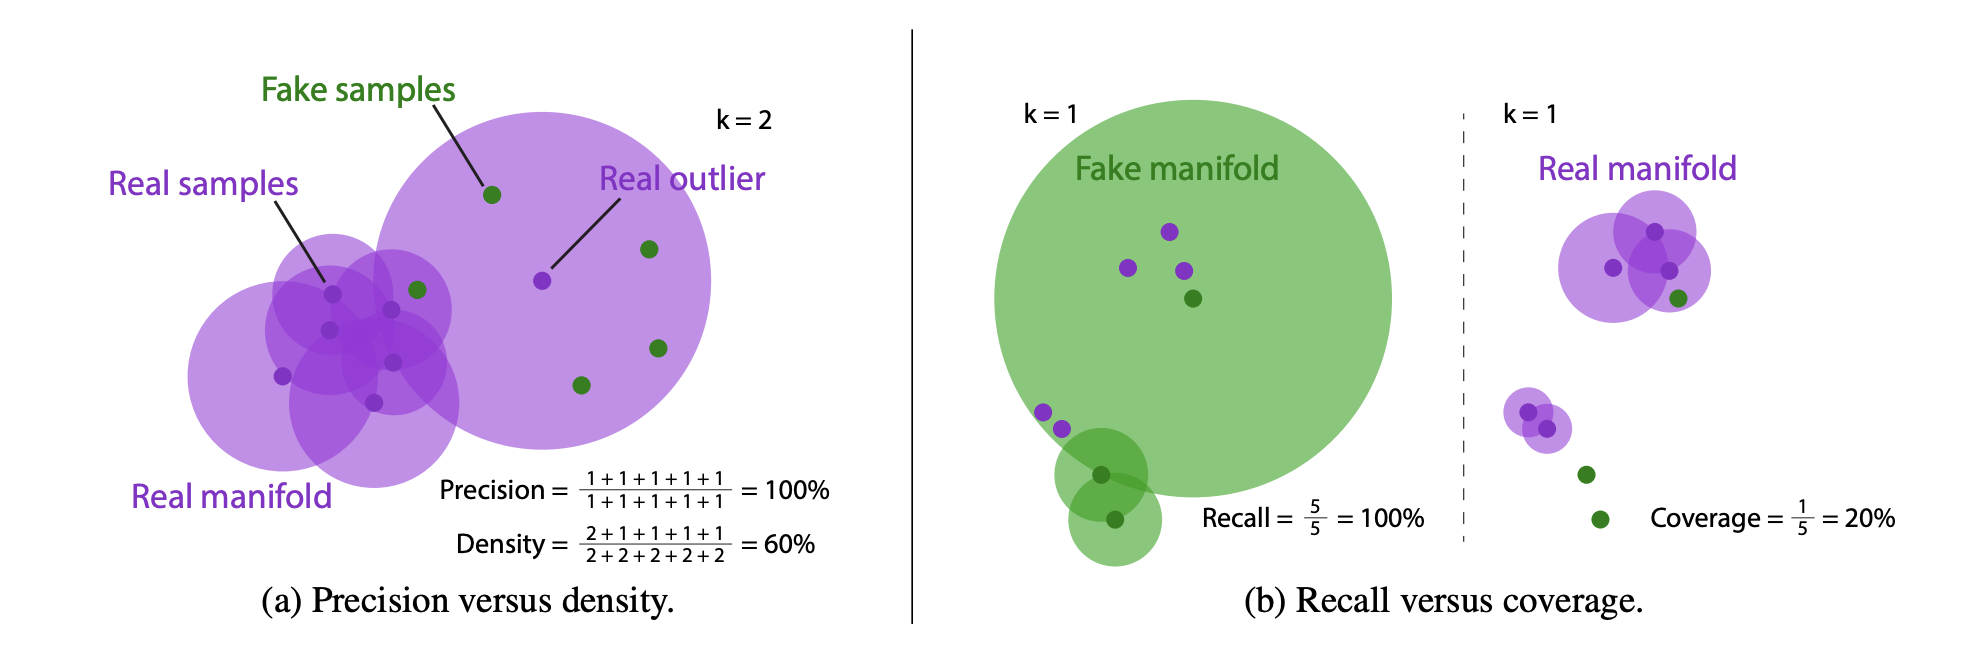
\includegraphics[width=15cm, height=7cm]{figs/precision_recall_coverage_density.png}
\caption{Two example scenarios for illustrating the advantage of density over precision and coverage over recall.
Note that for recall versus coverage figure, the real and fake samples are identical across left and right. Taken from article\cite{Coverage_Density}}
\label{fig:PrecisionRecallCoverageDensity}
\end{figure}
\subsection{Rarity score}
To calculalate 'rarity' of individual generation, Jiyeon el al. propose rariry score. They use KNN to represent manifold as Kynka¨anniemi et al.\cite{Precision_recall} make for precision and recall. Jiyeon writes: "We hypothesize that ordinary samples would be closer to each other whereas unique and rare samples would be sparsely located in the feature space"\cite[p.4]{RarityScore}. Formula of rarity score:
\begin{equation}
Rarity(\phi_g,\Phi_r)=\min_{r, s.t. \phi_g\in B_k(\phi_r,\Phi_r)}NN_k(\phi_r,\Phi_r)
\end{equation}
So, rarity score of a generated image is a radius of sphere of a
real images which contains the given generated image.

% \begin{longtable}{c|c}
% \caption[This is the title I want to appear in the List of Tables]{Simulation Parameters} \label{table:secsimulation_params} \\
% \hline
% A & B  \\
% \hline
% \endfirsthead
% \multicolumn{2}{@{}l}{} \\
% \hline
% A & B \\
% \hline
% \endhead
% \hline
%  \textbf{Parameter} & \textbf{Value}\\
%  \hline
%  Number of vehicles & $|\mathcal{V}|$\\
%  \hline
%  Number of RSUs & $|\mathcal{U}|$\\
%  \hline
%  RSU coverage radius & 150 m\\
%  \hline
%  V2V communication radius & 30 m\\
%  \hline
%  Smart vehicle antenna height & 1.5 m\\
%  \hline
%  RSU antenna height & 25 m\\
%  \hline
%  Smart vehicle maximum speed & $v_{max}$ m/s\\
%  \hline
%  Smart vehicle minimum speed & $v_{min}$ m/s\\
%  \hline
%  Common smart vehicle cache capacities & $[50, 100, 150, 200, 250]$ mb\\
%  \hline
%  Common RSU cache capacities & $[5000,1000,1500,2000,2500]$ mb\\
%  \hline
%  Common backhaul rates & $[75, 100, 150]$ mb/s\\
%  \hline
% \end{longtable}
\chapter{Methodology}
\label{chap:met}
In this chapter I provide description of improvement of current metrics. As I pointed in introduction I divided metrics on two types: distance metrics and score metrics. In distance metrics I change three aspects: feature extractor, distance computer and dataset on which metric is computing. In score metrics I change two aspects: feature extractor, dataset for finetuning of feature extractor. In this chapter I will describe the experiments I will conduct to evaluate the validity of the metric. Also I will provide new metric which would be somewhere in between distance metrics and score metrics.
\section{Distance metrics}
As I described in literature review FID consist of InceptionV3 as feature extractor and Fréchet Distance as distance metric which compute distance between two distributions: real images and generated images. So, I generalized diagram of FID from literature review chapter to distance metric at the Figure \ref{fig:DistanceMetric}:
\begin{figure}[hbt]
\centering
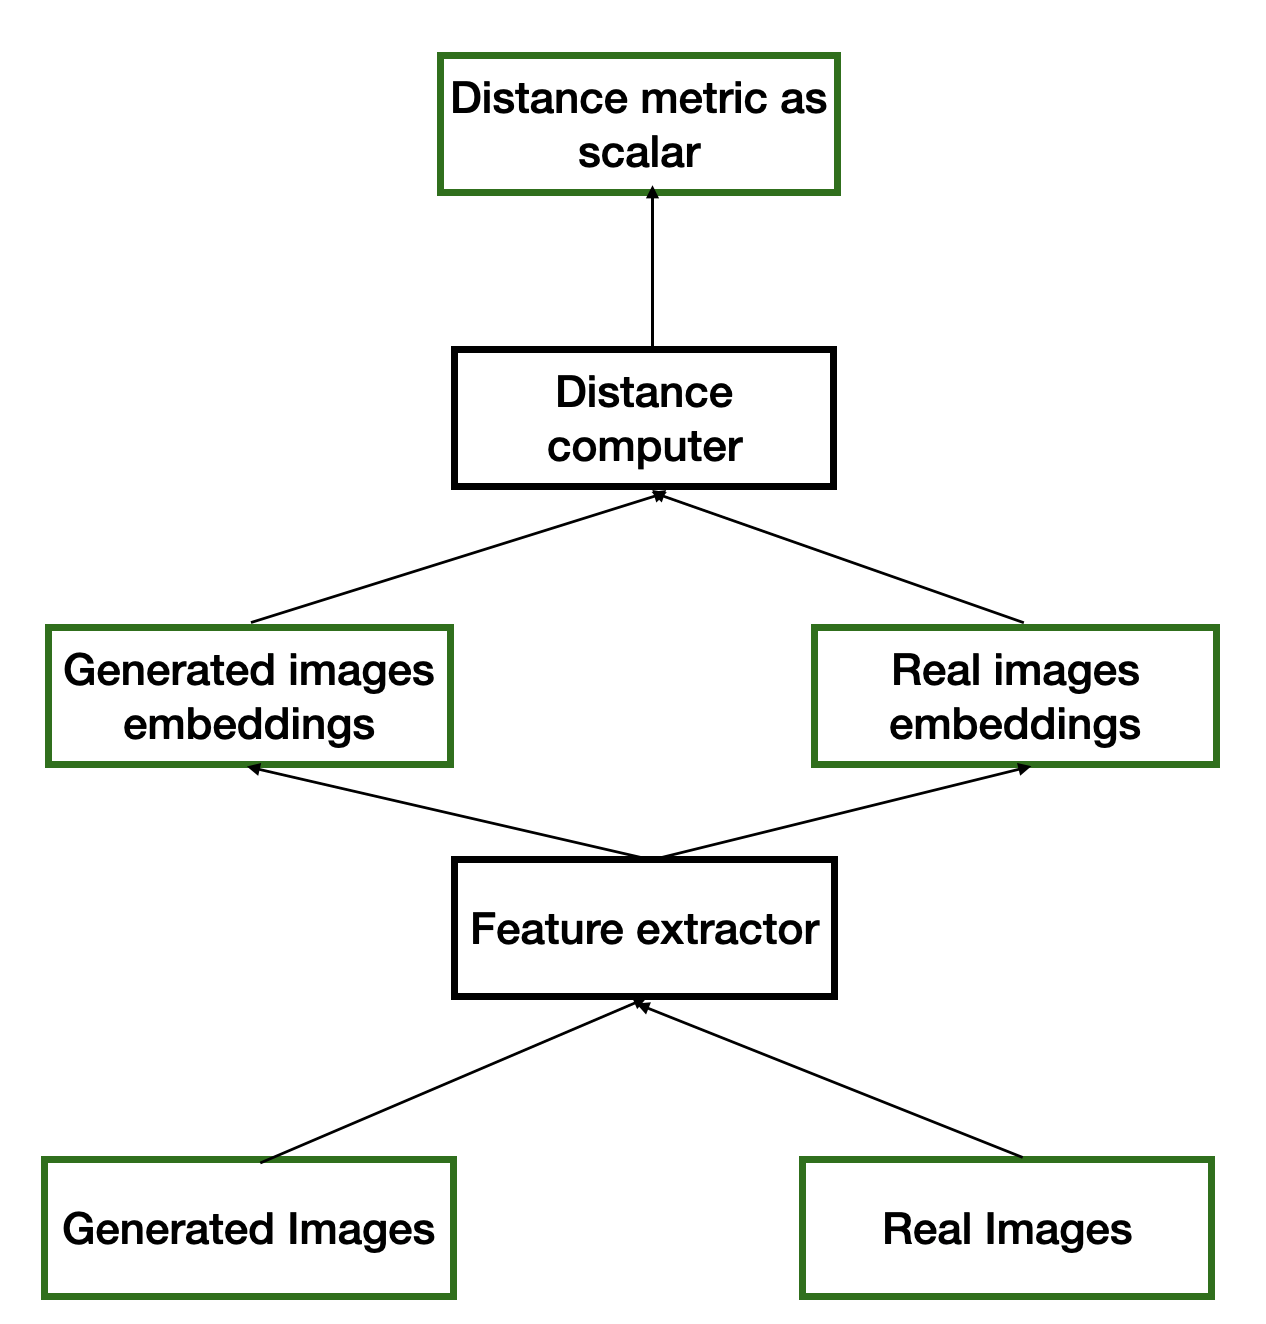
\includegraphics[width=8cm, height=10cm]{figs/distance_metric.png}
\caption{The diagram of distance metric}
\label{fig:DistanceMetric}
\end{figure}


The diagram shows that there are two components in the metric that can be changed: feature extractor - a model with which we extract features (embeddings) from images and distance computer - a formula that calculates the distance between embeddings of real and generated images. Actually, there's also a third component, which is a dataset of real pictures and prompts. Prompts are used to generate pictures, and real pictures are used to calculate metrics.

\subsection{Feature extractor}
As feature extractor I use three models: InceptionV3, image encoder from CLIP architecture and DINOv2. DINOv2 and CLIP are a self supervised models. I sue self supervised models due to they better adaptability to new domains, better solving zero-shot problems and richer extracted features. I will not describe CLIP architecture here because I have already described it in the literature review chapter.
\subsubsection{DINOv2}
DINO\cite{DINO} develops the Siamese network approach with a momentum encoder update of one of the branches and introduces a view of this process as Knowledge distilation. 

Accordingly, the distilation takes place from teacher to student through cross-entropy of probability distributions. The student's weights are updated through the backprop mechanism, while the teacher's weights are updated through a moving average of the student's weights.

Mathilde Caron et al. \cite{DINO} replace BatchNorm with 2 procedures - centering and sharpening, which is essentially the same normalization, only the shift parameter in centering is updated via moving average. The authors describe the effect as follows: "centering prevents one dimension to dominate but encourages collapse to the uniform distribution, while the sharpening has the opposite effect"\cite[p.4]{DINO}. Mathilde Caron et al. \cite{DINO} use multicrop and show that increasing the number of local image patches improves the quality.
They also use this method to train the Transformer (ViT) and find an interesting effect - right out of the box, the network starts segmenting the image without any partitioning. And it does it better than supervised learning. I provide diagram of DINO model at the Figure~\ref{fig:DINO_dian}.
\begin{figure}[hbt]
\centering
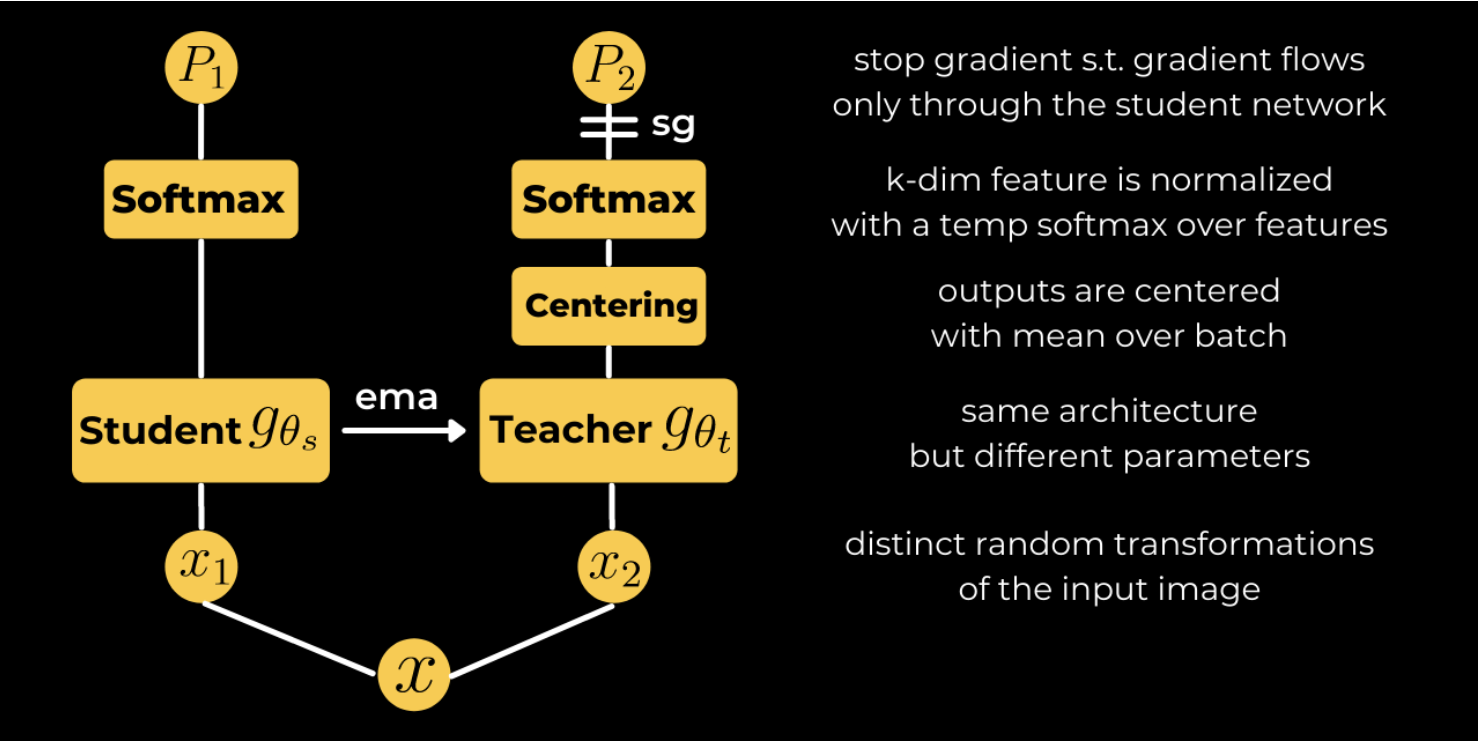
\includegraphics[width=15cm, height=10cm]{figs/DINO_diag.png}
\caption{Diagram of DINO}
\label{fig:DINO_dian}
\end{figure}

Also, I provide images and segmentation maps generated by DINO model and original images at the Figure~\ref{fig:DINO_seg_map}. I take it from original paper\cite{DINO}.
The figure shows how clearly DINO makes a segmentation map of the picture. DINOv2 is able to do higher-quality segmentation due to more careful and longer training.
\begin{figure}[hbt]
\centering
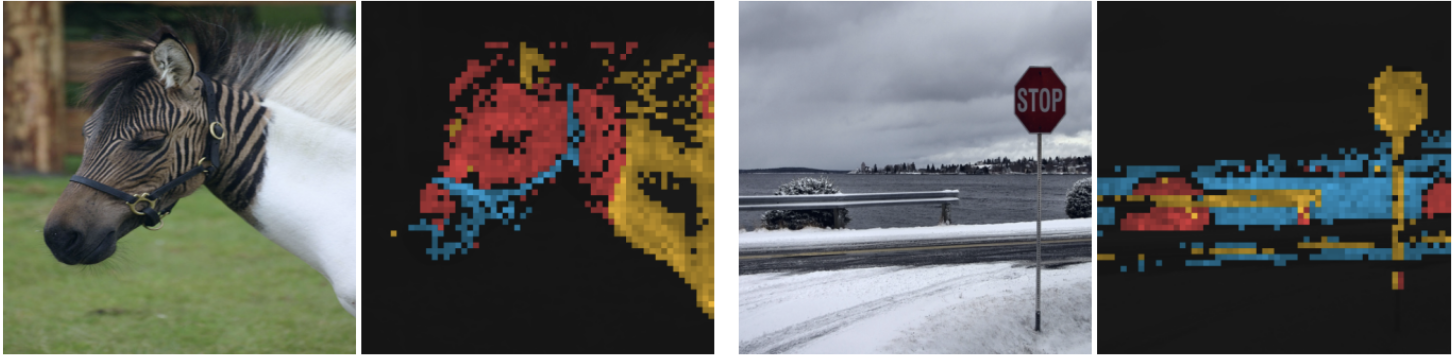
\includegraphics[width=15cm, height=5cm]{figs/DINO_seg_map.png}
\caption{Segmentation maps generated by DINO model and original images\cite{DINO}}
\label{fig:DINO_seg_map}
\end{figure}

DINOv2 is an improved version of DINO. DINOv2 generates not one feature for all images, but one feature for each 14*14 pixel square. This gives much more understanding of what is going on, and solves some of the CLIP problems.

\subsection{Distance computer}
As distance computer I choose tho methods: fréchet distance(FD) and kernel distance(KD). Kernel distance is also called maximum mean discrepancy(MMD). I choose FD due to it is standard distance computer function in such metric as FID and KD due to it is promising method which does not make assumtion about normality of distribution in contrast to FD.
\subsubsection{Kernel Distance}
In the following under kernel distance(KD) and maximum mean discrepancy I will have the same thing. I got the idea of using KD as a formula for calculating the distance between distributions from an article that uses KD together with embeddings from CLIP\cite{KD_CLIP}.

KD is described using the following formula:
\begin{equation}
dist^2(P,Q)=\mathbb{E}_{x,x'}[k(x,x')] + \mathbb{E}_{y,y'}[k(y,y')] -2\mathbb{E}_{x,y}[k(x,y)]
\end{equation}
Sadeep et al. provide information:"$x$ and $x'$ are independently distributed by $P$ and $y$ and $y'$ are independently distributed by $Q$"\cite[p.5]{KD_CLIP}.
If we have two datasets, $X={x_1,x_2,...,x_m}$ sampled from $P$ and $Y={y_1,y_2,...,y_m}$ sampled from $Q$, then unbiased estimator will be
\begin{equation}
\begin{split}
dist^2(X,Y)=\frac{1}{m(m-1)}\sum_{i=1}^{m}\sum_{j\neq i}^{m}k(x_i,x_j)\\+\frac{1}{n(n-1)}\sum_{i=1}^{n}\sum_{j\neq i}^{n}k(y_i,y_j)\\-\frac{2}{mn}\sum_{i=1}^{m}\sum_{j=1}^{n}k(x_i,y_j)
\end{split}
\end{equation}
As the kernel I use the Gaussian kernel $k(x,y)=-\frac{||x-y||^2}{2\sigma^2}$. Advantages of KD over the FD are:
\begin{itemize}
    \item KD is distribution-free meaning that it does not require a normal distribution of images as FD.
    \item KD is unbiased.
    \item KD is efficient from a computational point of view, since it does not require the computation of large matric as FD requires.
\end{itemize}
\subsection{Dataset for evaluation}
The dataset is very important for calculating the metric, as the actual images from the dataset determine what we should be aiming for with the generative model. I chose two datasets for my experiments:
\begin{enumerate}
    \item COCO with captions\cite{COCODataset}. it is 41 thousand real images. This is a standard dataset that is used to evaluate other metrics in other articles\cite{KD_CLIP}. In Figure\ref{fig:COCO_examples} it's possible to see that these are real images.
    \item MJHJ30K\cite{MJHQ30K}. This is a dataset of high-quality images generated with Midjourney with 10 common categories, each category with 3K samples. The difference of this dataset from COCO is that it contains not real, but more beautiful and aesthetic images. That is, it is better to use it if the model should generate aesthetic images similar to those generated by Midjourney. In Figure\ref{fig:MJHQ30k_examples} it's possible to see that the images are substantially different from those in COCO. The obvious differences are that the images in MJHQ30k are more aesthetically pleasing, more contrast and detailed.
\end{enumerate}

\begin{figure}[hbt]
\centering
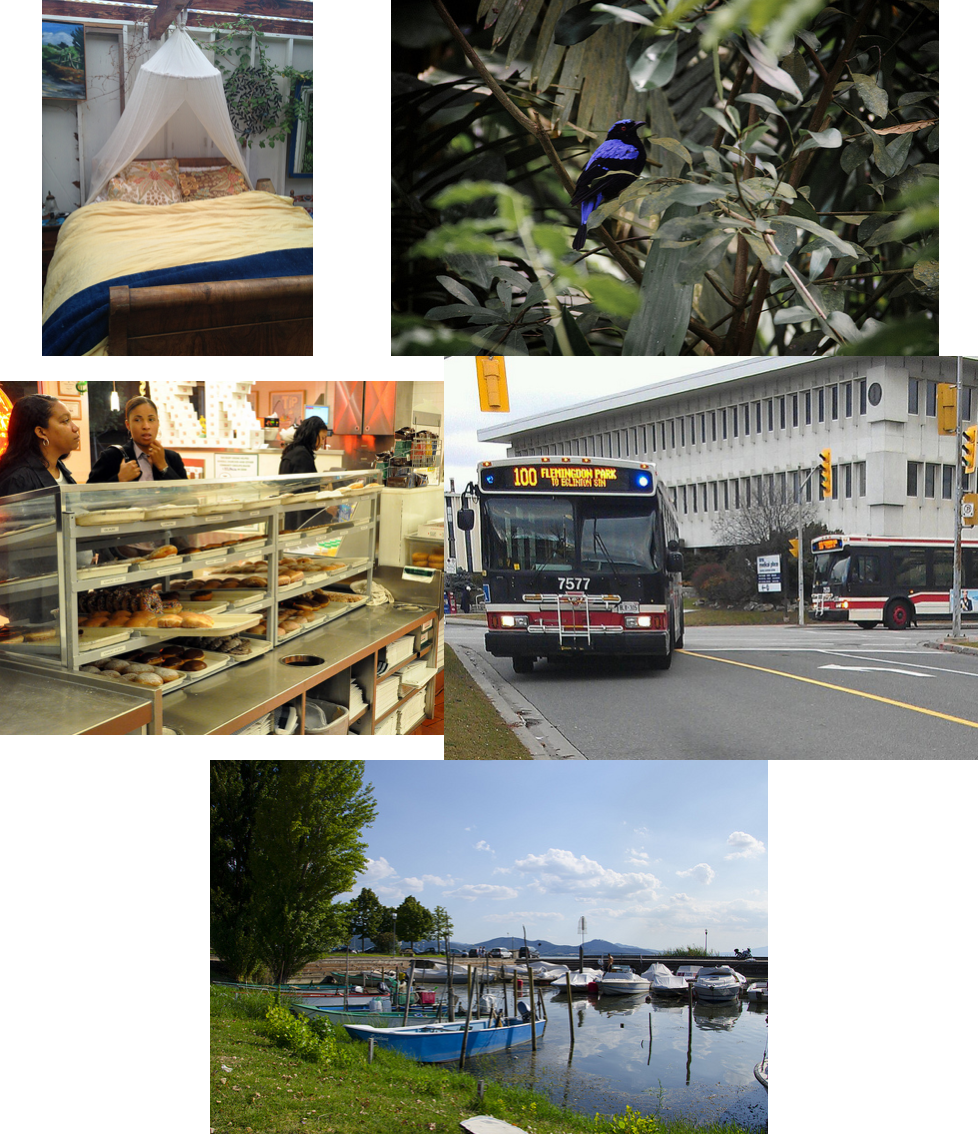
\includegraphics[width=7cm, height=10cm]{figs/coco_examples.png}
\caption{Images from COCO dataset with 41K real images}
\label{fig:COCO_examples}
\end{figure}

\begin{figure}[hbt]
\centering
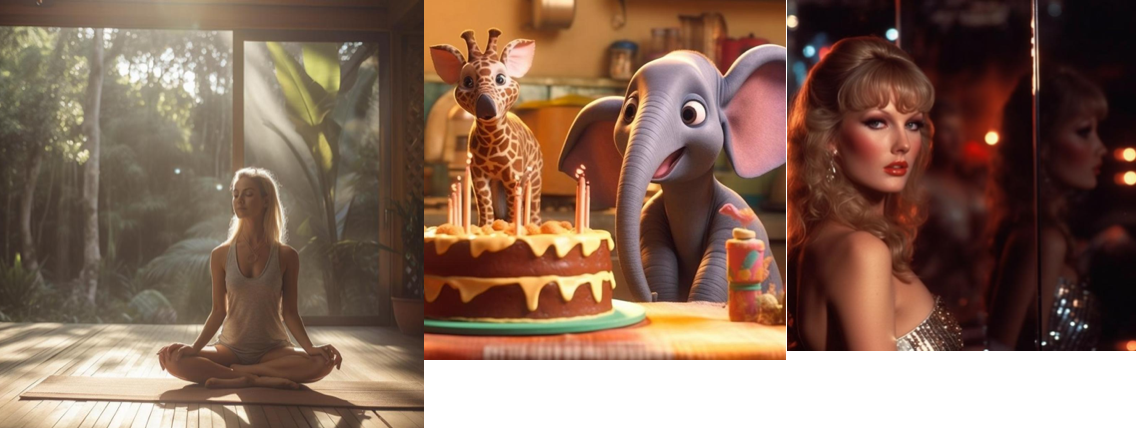
\includegraphics[width=12cm, height=5cm]{figs/mjhq30k_examples.png}
\caption{Images from MJHQ30K dataset with 30K generated by Midjourney and filted images}
\label{fig:MJHQ30k_examples}
\end{figure}

\subsection{Summary}
In conclusion, I chose three different models as feature extractor, two methods as distance computer and two datasets. This adds up to a total of 12 different metrics.\\
\begin{table}[h]
\centering
\begin{tabularx}{0.8\textwidth} { 
  | >{\centering\arraybackslash}X 
  | >{\centering\arraybackslash}X 
  | >{\centering\arraybackslash}X | }
 \hline
  & Kernel Distance(KD) & Fréchet Distance(FD) \\
 \hline
 InceptionV3  & KID  & FID  \\
 \hline
 CLIP  & KD\_CLIP  & FD\_CLIP  \\
\hline
 DINOv2  & KD\_DINOv2  & FD\_DINOv2  \\
\hline
\end{tabularx}
\caption{Distance metrics}
\label{tab:distance_metrics}
\end{table}
\section{Score metrics}
Idea behind each score metric is to extract
features(embeddings) from prompt and generated image and calculate simmula-
rity between two embeddings. Resulting scalar will be result of the metric. For the results of such a metric to be correct, it is necessary to be sure that the embeddings of the image and the prompt are in the same vector space. This property is represented by CLIP\cite{CLIP} and its variants such as BLIP\cite{BLIP}. The diagram of score metric is shown at the Figure\ref{fig:Score_metric}.
\begin{figure}[hbt]
\centering
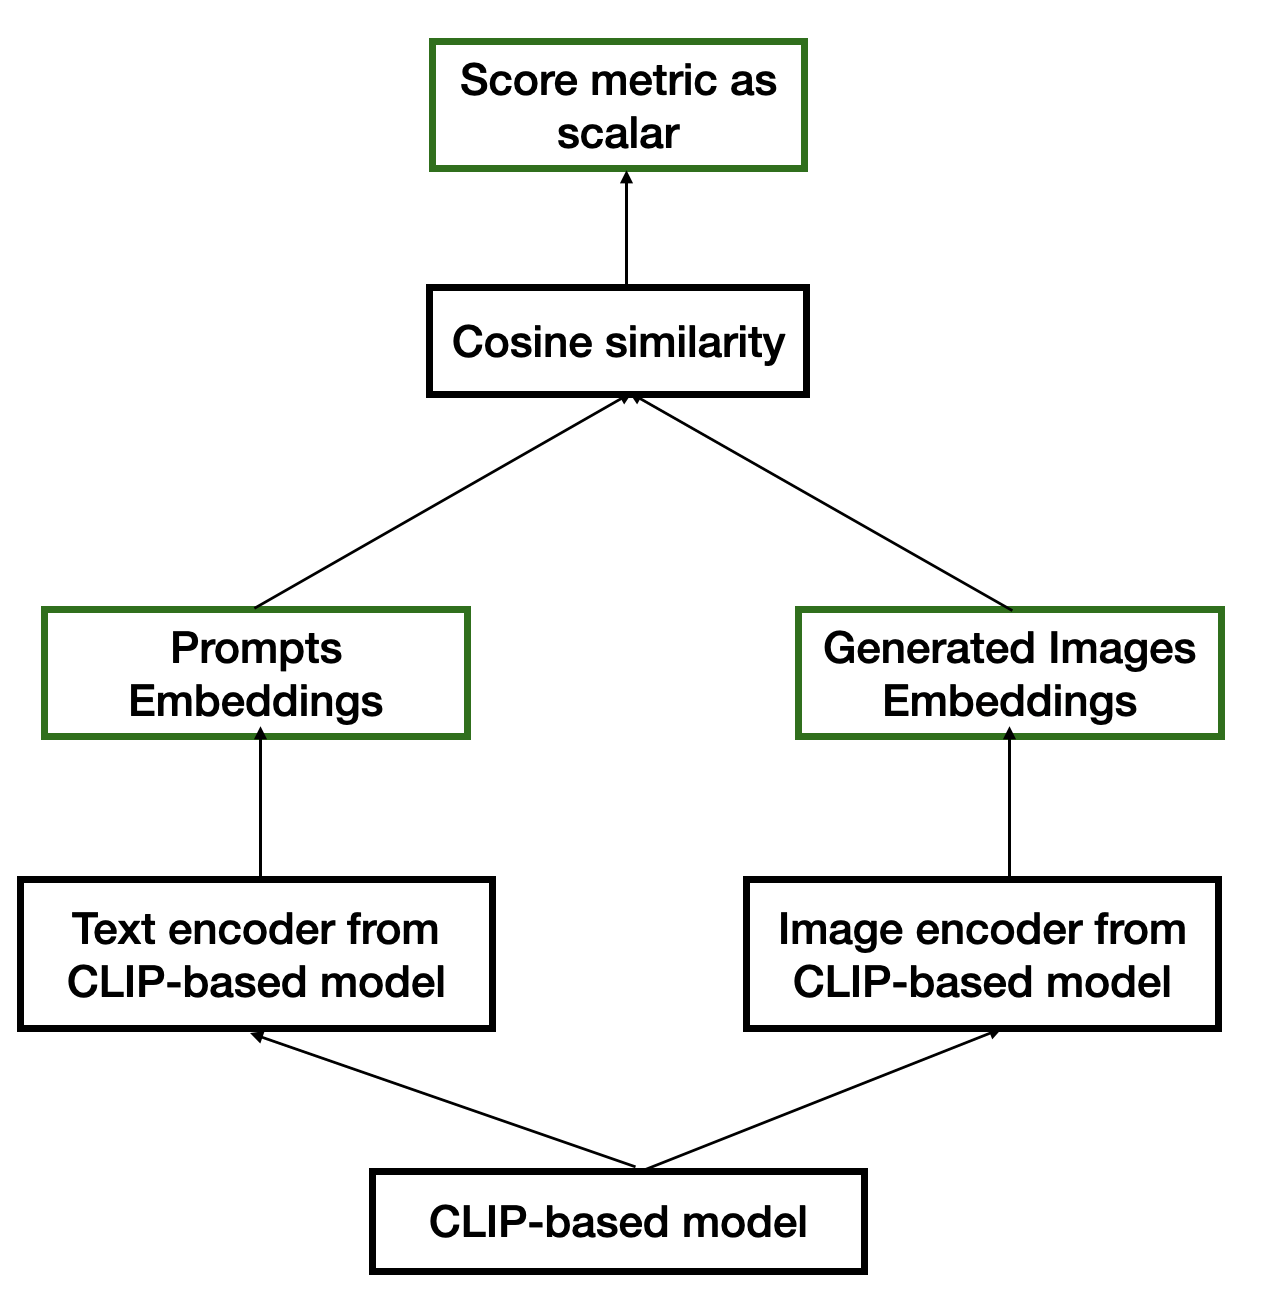
\includegraphics[width=8cm, height=10cm]{figs/score_metric.png}
\caption{Diagram of score metric}
\label{fig:Score_metric}
\end{figure}
I'll be using the following score metrics:
\begin{enumerate}
    \item ClPPscore\cite{CLIPScore} - standard metric.
    \item MCLIPScore - CLIPSore but with MCLIP instead CLIP.
    \item ImageReward\cite{Image_reward}.
    \item HPSv2\cite{HPSv2}.
\end{enumerate}
\subsection{MCLIPScore}
Idea is the same as in CLIPScore which I descibed in literature review chapter, but MCLIP is used instead of CLIP.

Unlike CLIP, which learns and works predominantly with English, MLIP learns and is able to interpret texts in different languages, which improves its applicability globally.
\subsection{ImageReward}
Idea of ImageReward\cite{Image_reward} is to use BLIP architecture with modification and make new dataset for finetuning. Jiazheng et al.\cite{Image_reward} take the features from prompt and image using BLIP, combine them using Cross-Attention and using linear layer make a scalar to get the score.
\subsubsection{BLIP}
The main goal of BLIP (Bootstrapped Language Image Pretraining) is to improve the model's ability to interact between language and visual content.


While CLIP is trained using contrastive learning, which aims at converging vector representations of images and corresponding textual descriptions, BLIP introduces additional tactical strategies, such as self-distillation, to improve the stability of learning and the quality of the representations generated by the model. Self-distillation is a technique where knowledge from one part of the model is transferred to another part of the model, improving its overall performance and generalization ability.
\subsubsection{ImageReward Dataset}
Jiazheng et al. used DiffusionDB: a prompt and image database created with Stable Diffusion. DiffusionDB stores 1.8M data which is too much, so certain prompts are selected using the following algorithm:
\begin{enumerate}
    \item Prompts are encoded using Sentence-BERT and KNN is constructed with cosine similarity as distance.
    \item Score of each vertex is formed as the number of neighbors which are not selected.
    \item Vertices are selected based on score and then score is recalculated.
    \item Since the complexity is quadratic, the dataset is divided into 100 sets (20k prompts in each set) and 100 prompts are selected in each set -> 10k diverse prompts in the end.
\end{enumerate}
Further, to finetune on this dataset the model it was necessary to assign to each pair of generated image-prompt some score. For this purpose, people were involved who evaluated pairs on a 7-ball scale of aesthetics, relevance and defectiveness.

ImageReward model is funetuned using the following formula:
\begin{equation}
loss(\theta)=-\mathbb{E}[log(\sigma(f_\theta(T,x_i) - f_\theta(T,x_j)))]
\end{equation}
where $T$ is a prompt and $x_i$ is a image that better then $x_j$ image.
\subsection{HPSv2}
The idea behind HPSv2\cite{HPSv2} is to make your own dataset and finetune CLIP on it.
\subsubsection{Dataset collecting}
Prompts are taken from two datasets “COCO Captions” and “DiffusionDB” cleaned with chatGPT.

Xiaoshi et al. take different model patterns and generate a picture of each pattern for each prompt. Also for the prompts from “COCO Captions” real pictures are taken\cite{HPSv2}.

The test data is 400 groups. Of them 300 groups from DuffusionDB generated by 9 models and 100 groups from COCO Captions generated by 9 models and plus one real picture from COCO Captions. Total 10 anonators per group: 300 * (9 * 8 / 2) * 10 + 100 * (10 * 9 / 2) * 10 = 300 * 360 + 45000 = 108000 + 45000 = 153000 binary comparisons.


Train data is 107,515 groups. Each group is 4 pictures(coherent or real) and one anotator. 28,172 groups from COCO Captions the rest from DiffusionDB.

\subsubsection{Finetune process}
HPSv2 takes ViT-H/14 CLIP and fine-tune using the collected dataset. Train instance is two pictures $x_1$, $x_2$ of one prompt $p$ and $y=[1,0]$ if $x_1$ is better than $x_2$. CLIP score is counted with temperature(trained parameter):
\begin{equation}
s_\theta(p,x)=\frac{Enc_{txt}(p)*Enc_{img}(x)}{\tau}
\end{equation}
Predicted preference is calculated as:
\begin{equation}
\hat{y_i}=\frac{exp(s_\theta(p,x_i))}{\sum_{j=1}^{2}exp(s_\theta(p,x_j))}
\end{equation}
Then the training loss is:
\begin{equation}
L_{pref}=\sum_{j=1}^{2}y_i(log(y_i)-log(\hat{y_j}))
\end{equation}
Only the last 20 layers of image encoder and 11 layers of text encoder are trained.
\section{Human evaluation}
To determine a person's judgement I by themselves marked up mini datasets consisting of 300 samples, where a sample consists of a real picture, a prompt, and a generated picture. Such mini dataset was for each model used and for each dataset.

\section{Cosine similarity with DINOv2 features}
The problem with distance metrics is that they do not take into account in any way the information that the generated image and the real one refer to the same propmt. The problem with score metric is that it does not take into account the aesthetics of the picture as the metric simply does not include the aesthetic (real) picture to be based on.

I propose a method of computing metric that can anihilize both of these disadvantages. The idea of my metric is to take a feature extractor for each pair, extract the embeddings of the real and generated images and use cosine simularity to get the similarity of the two embeddings. To get a score for a dataset the arithmetic mean for each pair from the dataset is taken. The scheme of this metric would look like this:
\begin{figure}[hbt]
\centering
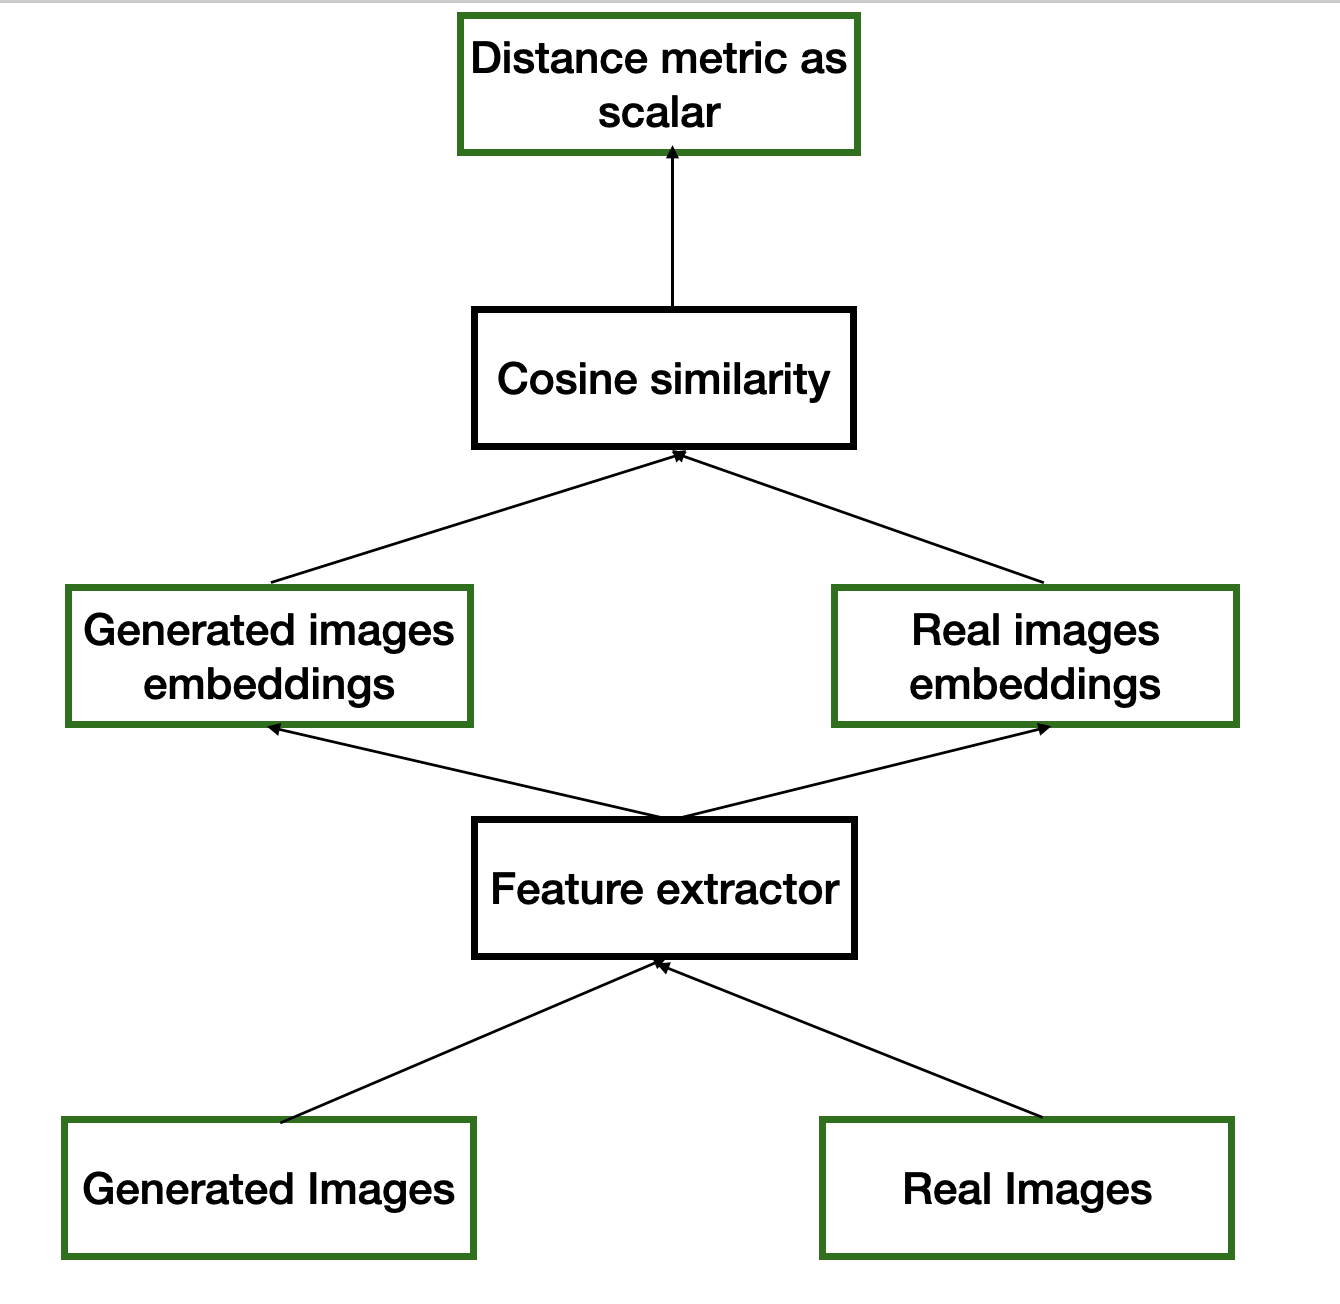
\includegraphics[width=8cm, height=10cm]{figs/cos_clip.png}
\caption{Diagram of my own metric, COS\_DINOv2}
\label{fig:cos_dinov2_diagram}
\end{figure}
It is possible to notice that the diagram is very similar to the distance metric. But it is important to note that to calculate distance in distance metric, some qualities are taken from embedding datasets, for example, mean and variance for FD or Gaussian kernel for KD. While in my method distance is calculated on embeddings for each pair directly.

I will use DINOv2 as a feature extractor in the experiments chapter in the future. I call such a metric COS\_DINOv2.
\chapter{Experiments}
In this chapter I will describe the experiments I conducted to evaluate the metrics. I will evaluate metrics of both classes: distance metric and score metric. Metrics such as FID, KID, FD\_CLIP, KD\_CLIP, FD\_DINOv2 and KD\_DINOv2 are distance metrics. While CLIPScore, ImageReward and HSPv2 are related to score metrics. All metrics will be evaluated on two datasets: COCO with 41 thousand samples and MJHQ30k with 30 thousand samples.

I will use the Imagen\cite{Imagen} diffusion model for my experiments.I will conduct the following experiments:
\begin{enumerate}
    \item Measure the quality of the model at different steps of image generation.
    \item Measure the quality of the model at different iterations of model training.
    \item Measure the quality of the model with corrupted images by overlaying black squares on the images.
\end{enumerate}
In what follows I will describe each experiment in more detail and will attach graphs and measurement results.

And it is important to note that distance metrics which used CLIP as feature extractor was measured two times: with normalized featured and without. Normalized features are marked as "CLIP\_norm", not normalized just "CLIP".
\section{Imagen}
First, I want to describe the structure of the Imagen\cite{Imagen} diffusion network. Imagen is a state-of-the-art text-to-image generation model developed by researchers at Google Research, announced in May 2022.

Imagen's diffusion model successively adds noise to an image over a series of steps until the data is completely random (pure noise). Starting from noise, the model learns to gradually denoise the data, reconstructing an image conditioned on the given text input. This is achieved through a series of learned de-noising steps.


Imagen leverages a Transformer-based \cite{Visual_transformer} architecture for conditioning on text. This allows for capturing complex relationships and semantic details from the text, integrating these into the image synthesis process more effectively than previous models like DALL-E \cite{DALLE}.

Different from some prior models, Imagen produces high-fidelity and high-resolution images by utilizing a super-resolution process. This involves generating an image at a relatively lower resolution initially and then progressively enhancing its details and resolution in subsequent stages. In summary, the essence of Imagen's diffusion model is the sophisticated use of textual description-based noise introduction and removal processes to create high-resolution photorealistic images.

In conclusion, Imagen has several distinguishing features:
\begin{enumerate}
    \item The use of a large encoder for text compared to the weight and size of the diffusion model.
    \item The use of frozen text encoder.
    \item The use of two additional diffusion models to improve image quality. These diffusion models are called "Super-Resolution Diffusion Model".
\end{enumerate}
Figure \ref{fig:Imagen_diagram} \cite{Imagen} taken from the original article shows the structure of the Imagen diffusion model.
\begin{figure}[h]
\centering
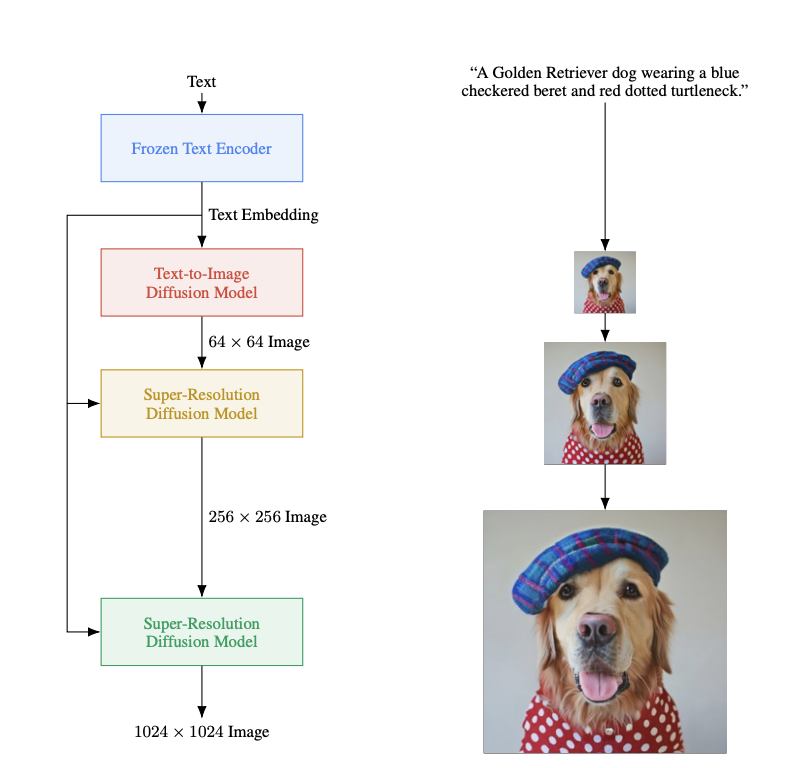
\includegraphics[width=12cm, height=12cm]{figs/Imagen_diagram.png}
\caption{Imagen diagram taken from \cite{Imagen}. Chitwan Saharia et al. highlights: "Imagen uses a frozen text encoder to encode the input text
into text embeddings. A conditional diffusion model maps the text embedding into a 64 × 64 image.
Imagen further utilizes text-conditional super-resolution diffusion models to upsample the image,
first 64 × 64 → 256 × 256, and then 256 × 256 → 1024 × 1024."\cite[p.19]{Imagen}}
\label{fig:Imagen_diagram}
\end{figure}

\section{Experiments with distance metrics}
\subsection{Different iterations of model training}
The first experiment I did was to train Imagen with different numbers of training steps, i.e. some models were undertrained. The intuition is that the image obviously gets better and better with more training steps. I purposely made a small number of steps so that the model would not have time to overtrain. I got several models: Imagen trained at 100K, 150K, 200K and 300K training steps.

I took the COCO dataset and measured the metrics on it. I plotted all distance metrics at Figure \ref{fig:coco_train_steps}. The metric correlates more strongly with human judgment if the red and blue graphs match.
The results I got from the graphs:
\begin{itemize}
    \item FID and KID correlate with human judgement well enough if metrics are calculated on COCO dataset.
    \item KD\_CLIP, FD\_CLIP, KD\_CLIP\_norm, FD\_CLIP\_norm acting weird, so there's no pattern.
    \item FD\_CLIP and FD\_CLIP\_norm are similar. KD\_CLIP and KD\_CLIP/norm are also similar
    \item FD\_DINOv2 correlates with human opinion better than any other metric.
    \item KD\_DINOv2 is completely different from a person's opinion.
\end{itemize}

I took the MJHQ30K dataset and measured the metrics on it. I plotted all distance metrics at Figure \ref{fig:mjhq30k_train_steps}. The metric correlates more strongly with human judgment if the red and blue graphs match.
The results I got from the graphs:
\begin{itemize}
    \item FID and KID correlate with human judgement well enough if metrics are calculated on MJHQ30K dataset.
    \item KD\_CLIP, FD\_CLIP, KD\_CLIP\_norm, FD\_CLIP\_norm acting weird, so there's no pattern.
    \item FD\_CLIP and FD\_CLIP\_norm are similar. KD\_CLIP and KD\_CLIP/norm are also similar
    \item FD\_DINOv2 and KD\_DINOv2 correlates with human opinion better than any other metric.
\end{itemize}

\begin{figure}[]
\centering
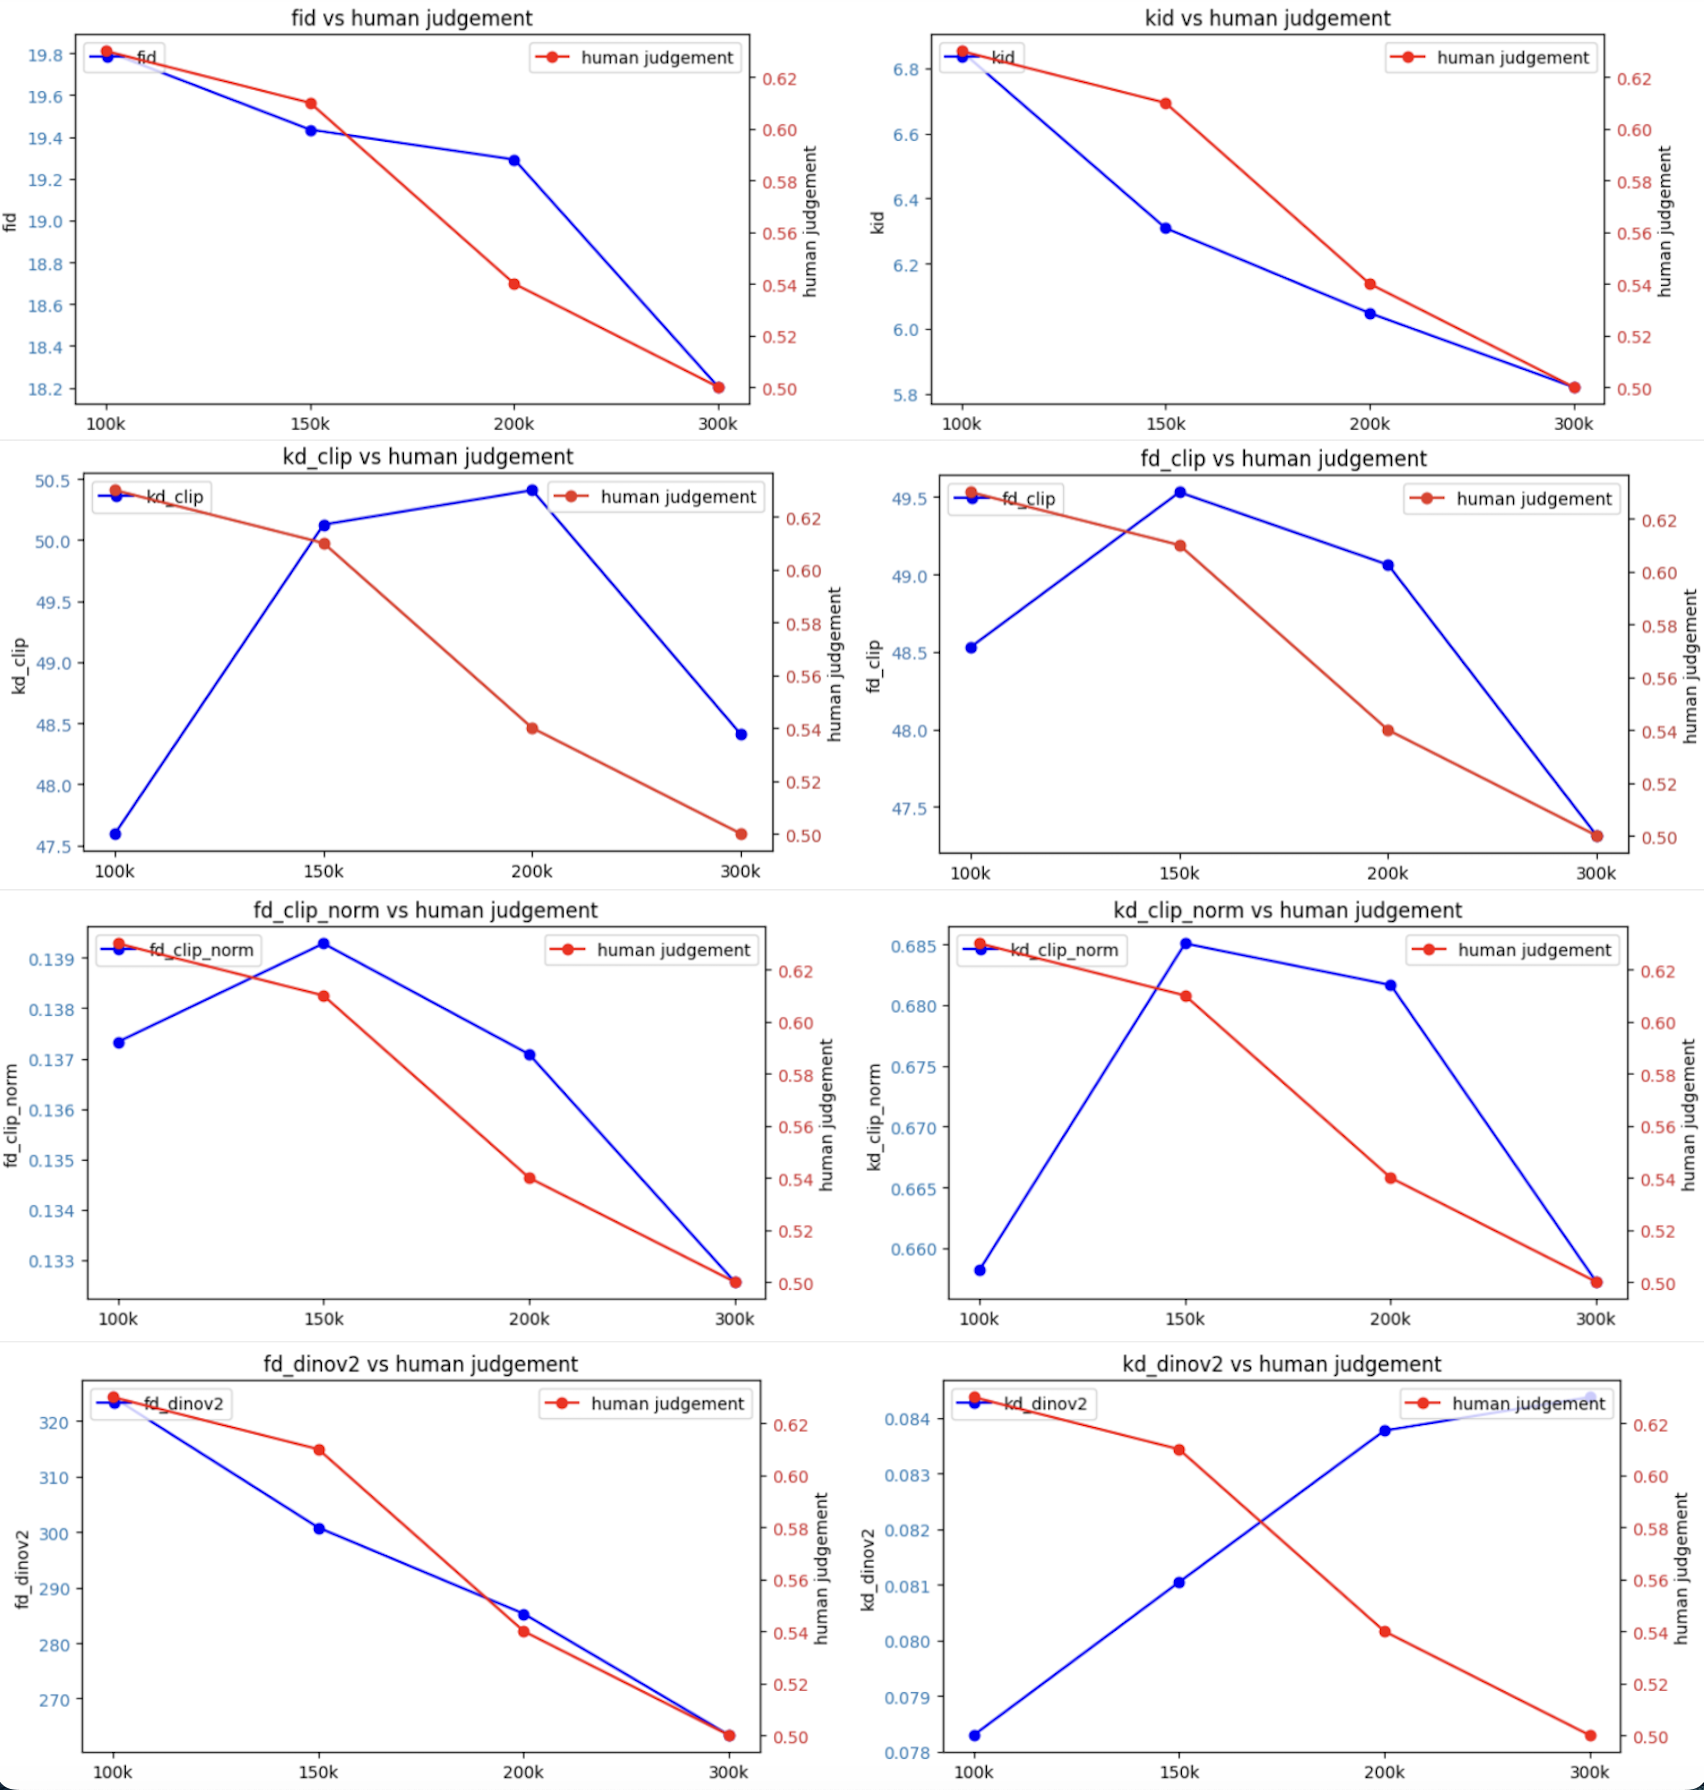
\includegraphics[width=16cm, height=17cm]{figs/coco_train_steps.png}
\caption{Distance metrics measured on COCO dataset on models with different number of train steps. On the X-axis from left to right there are models with different number of steps from smaller to larger, i.e. from 100 thousand to 300 thousand. The left Y-axis shows the results of the metric, so the blue graph corresponds to the left Y-axis. On the right Y-axis are the results of human evaluation - this is the proportion of victories of the fully trained model (i.e. the model with 300 training steps) against the current model with the current number of training steps. The red graph corresponds to the right Y-axis.}
\label{fig:coco_train_steps}
\end{figure}

\begin{figure}[]
\centering
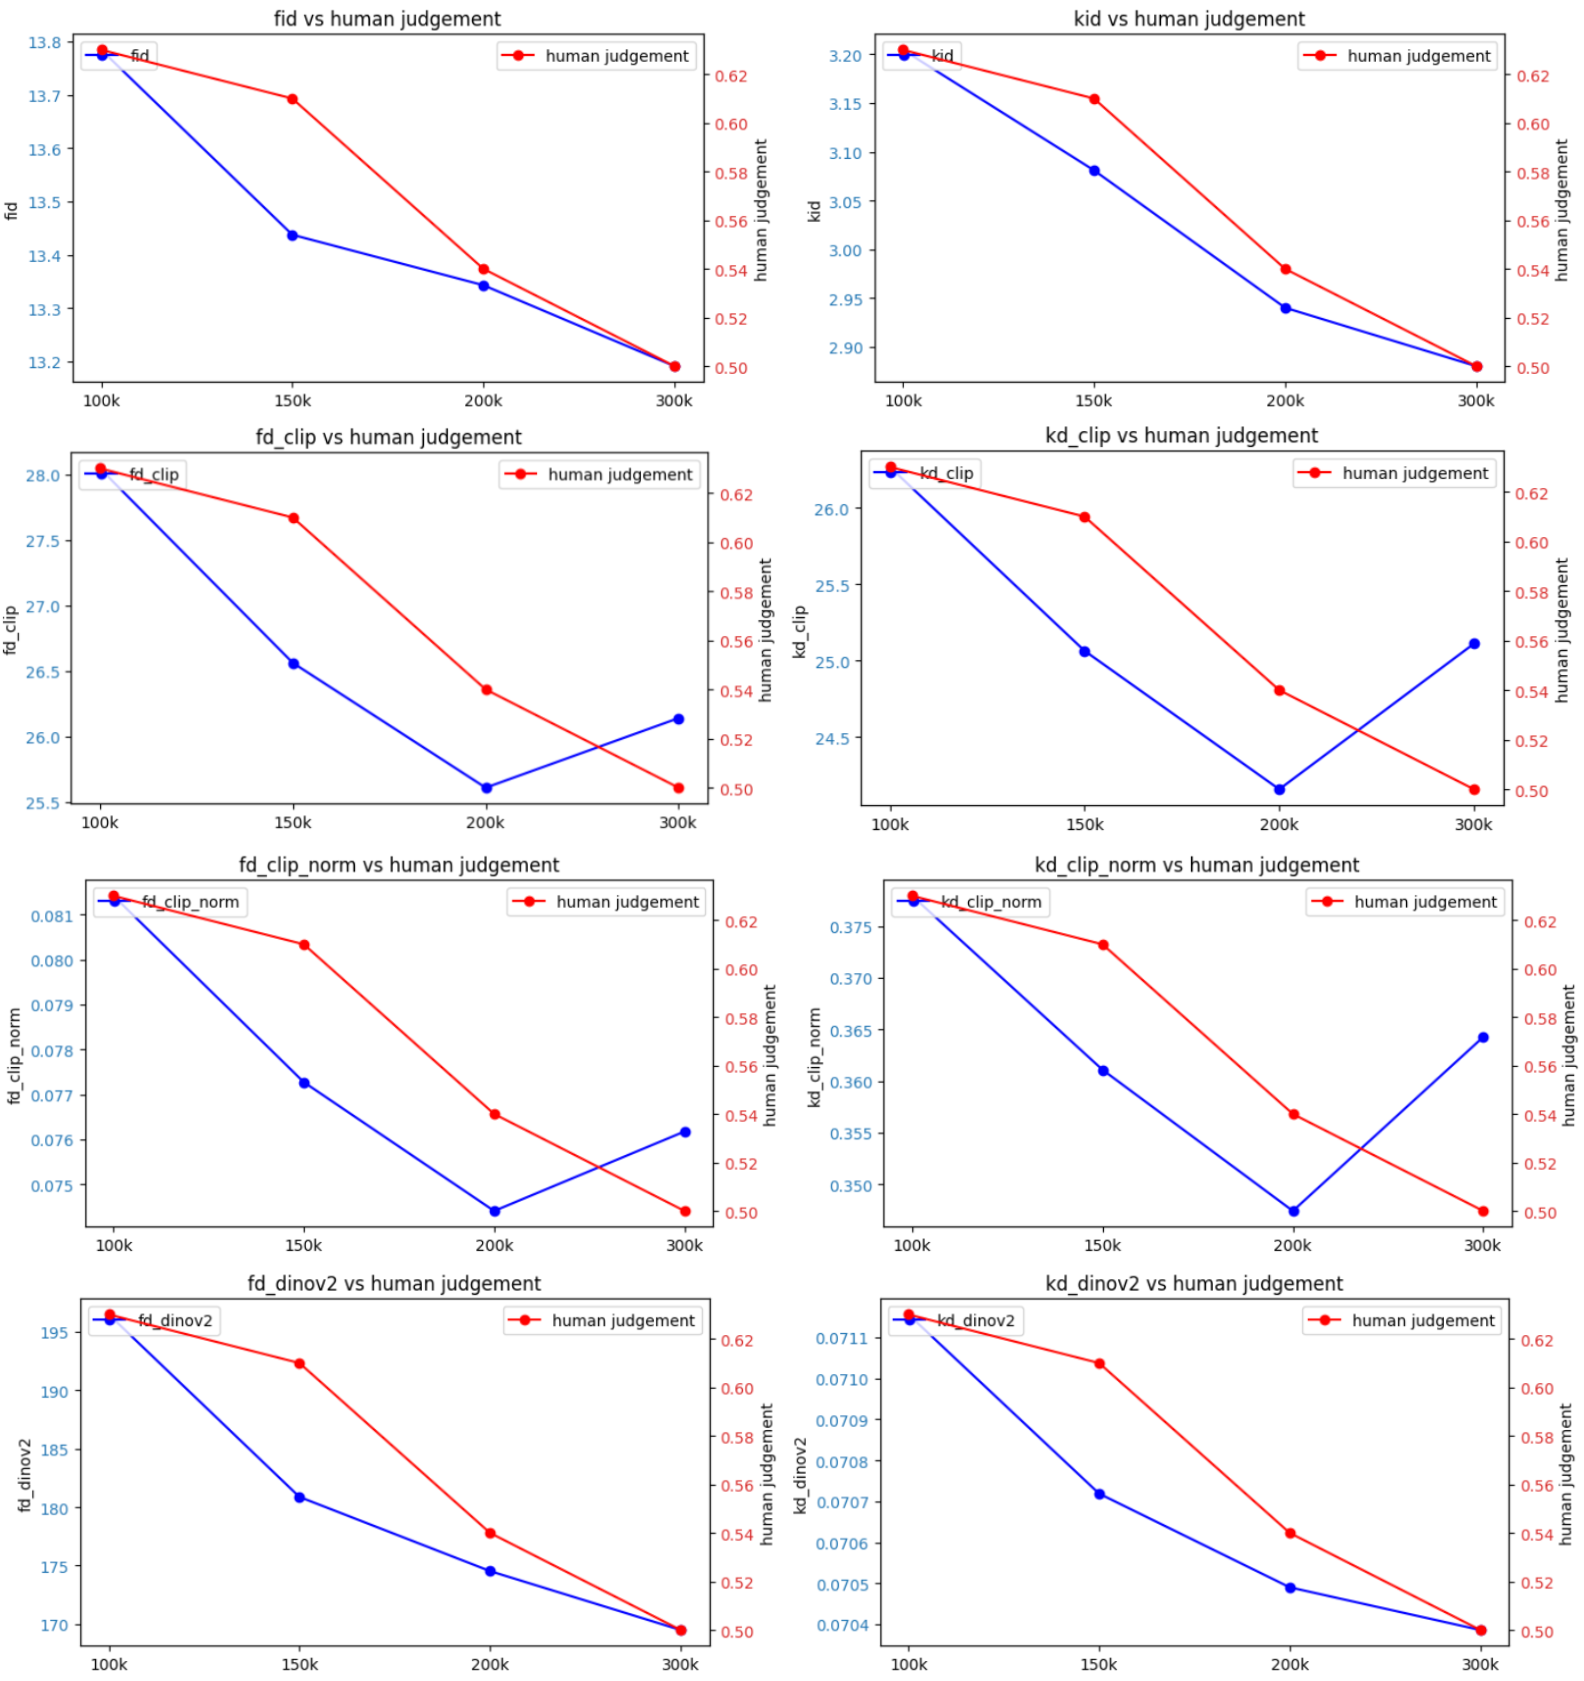
\includegraphics[width=16cm, height=17cm]{figs/mjhq30k_train_steps.png}
\caption{Distance metrics measured on MJHQ30K dataset on models with different number of train steps. The axes are the same on the Figure\ref{fig:coco_train_steps}.}
\label{fig:mjhq30k_train_steps}
\end{figure}

\subsubsection{Summary}
At the end of this experiment I can say that the FD\_DINOv2 metric performed the best. FID and KID also showed excellent results. FD\_CLIP, KD\_CLIP, FD\_CLIP\_norm and KD\_CLIP\_norm show poor results which may doubt CLIP as feature extractor. KD\_DINOv2 showed excellent results on the MJHQ30k dataset, but the exact opposite on COCO.

I have an assumption that this behavior may be due to the fact that the model generates images more similar to the images that MJHQ30K generates, i.e. contrast and aesthetics, than to the real images that are in the COCO dataset.

\subsection{Different steps of image generation}
The second experiment I did was to take the trained Imagen model and generate an image, but at different generation steps, i.e. at different de-noising steps. The intuition is that the image obviously gets better and better with more de-noising steps.

I took the COCO dataset and measured the metrics on it. I plotted all distance metrics at Figure \ref{fig:coco_gen_steps}. The metric correlates more strongly with human judgment if the red and blue graphs match.
The results I got from the graphs:
\begin{itemize}
    \item FID correlate with human judgement well enough if metrics are calculated on COCO dataset.
    \item KID, KD\_CLIP, FD\_CLIP, KD\_CLIP\_norm, FD\_CLIP\_norm acting weird, so there's no pattern.
    \item FD\_CLIP and FD\_CLIP\_norm are similar. KD\_CLIP and KD\_CLIP/norm are also similar
    \item FD\_DINOv2 correlates with human opinion better than any other metric.
    \item KD\_DINOv2 is completely different from a person's opinion, as the last experiment.
\end{itemize}

I took the MJHQ30K dataset and measured the metrics on it. I plotted all distance metrics at Figure \ref{fig:mjhq30k_gen_steps}. The metric correlates more strongly with human judgment if the red and blue graphs match.
The results I got from the graphs:
\begin{itemize}
    \item All metrics correlate with human judgement well enough if metrics are calculated on MJHQ30K dataset.
\end{itemize}

\begin{figure}[]
\centering
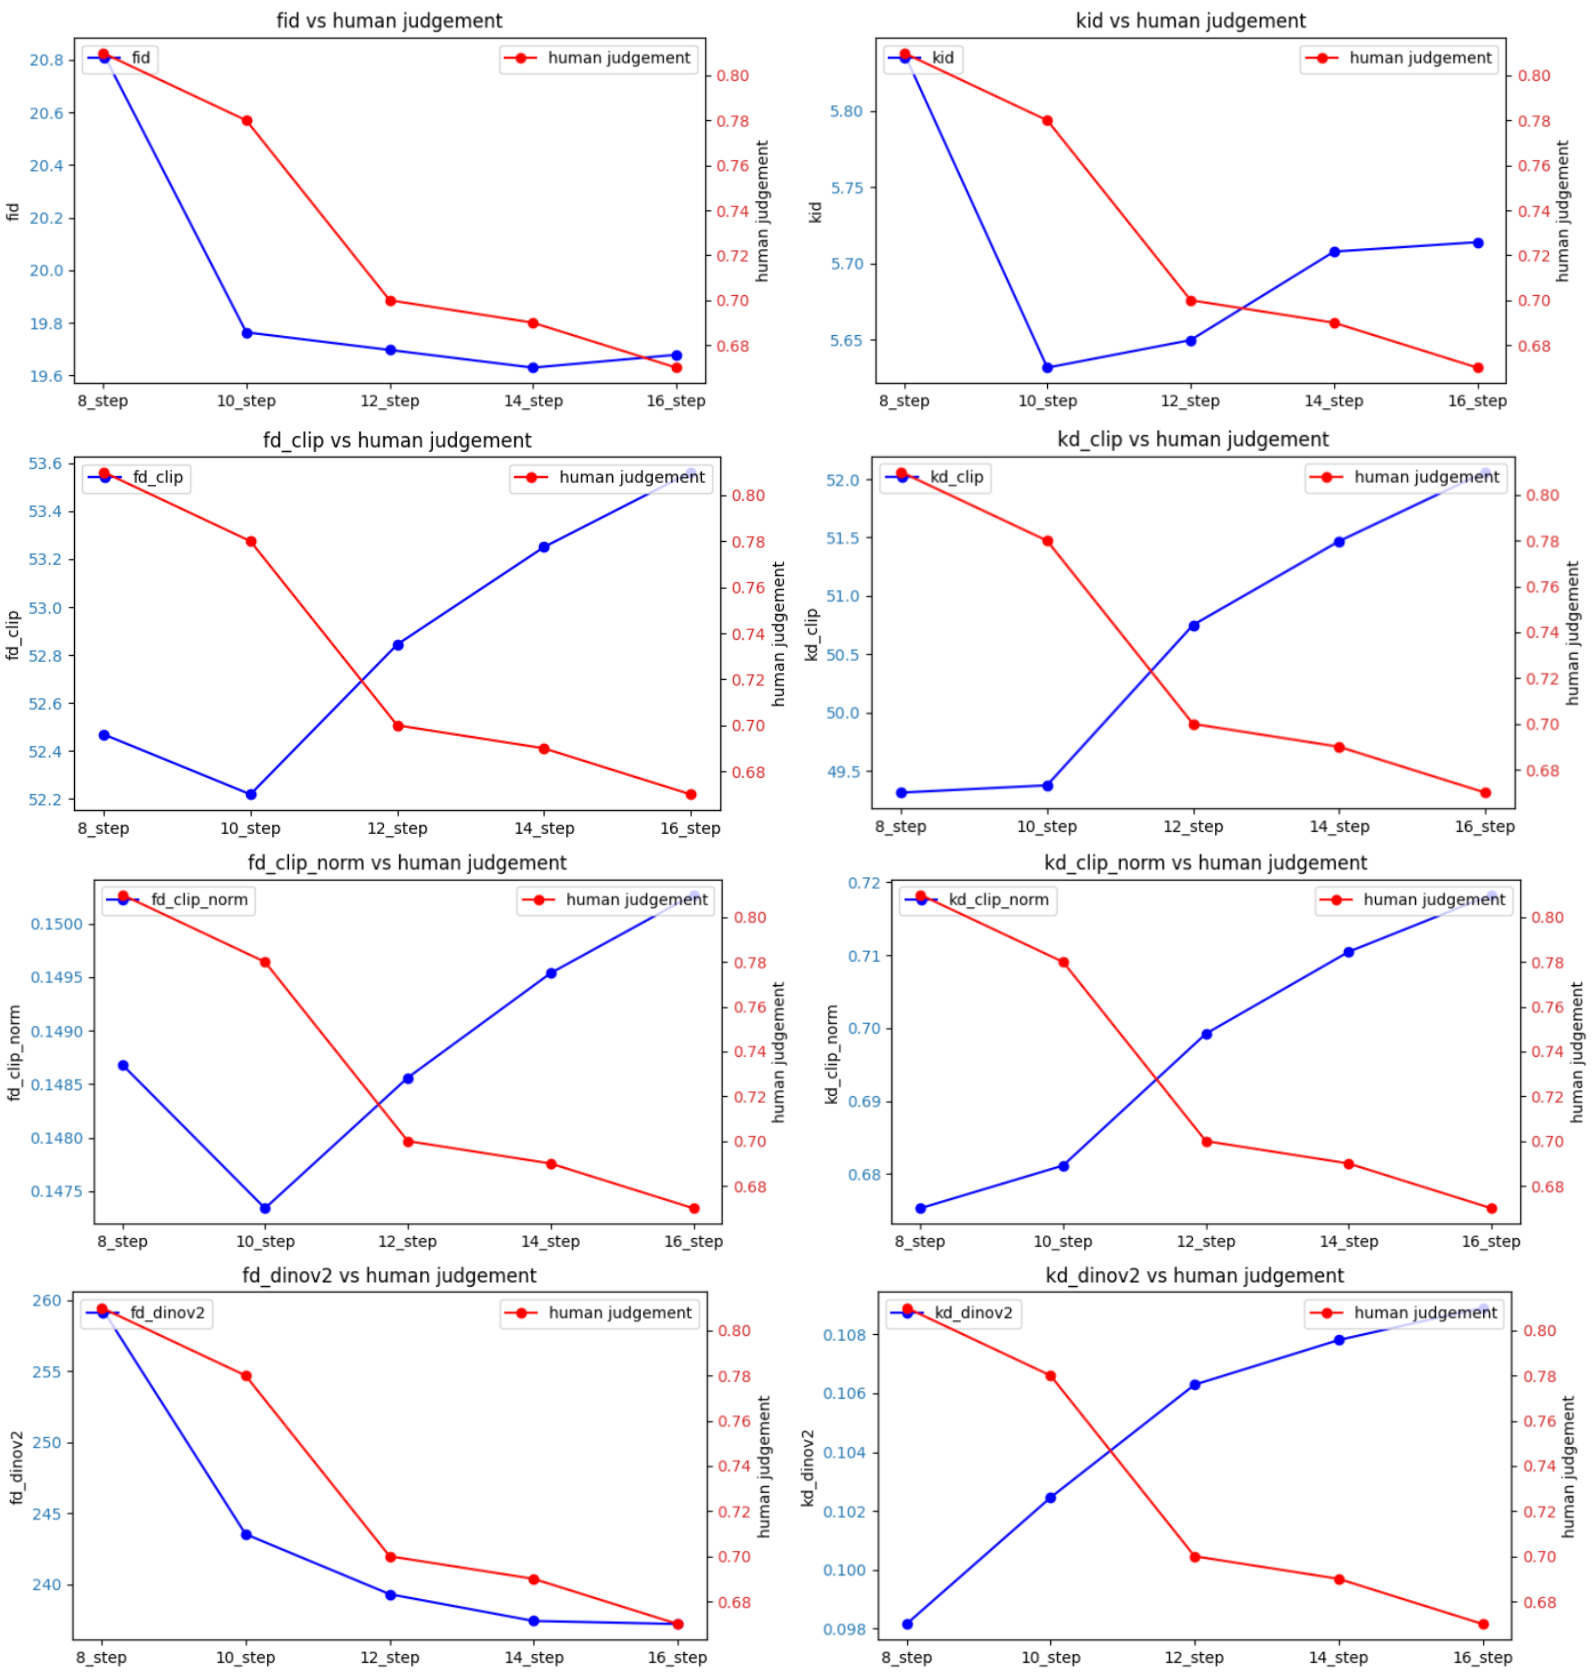
\includegraphics[width=16cm, height=17cm]{figs/coco_gen_steps.png}
\caption{Distance metrics measured on COCO dataset on models with different number of de-noising(generation) steps. On the X-axis from left to right there are models with different number of steps from smaller to larger, i.e. from 8 steps to 16 steps. The left Y-axis shows the results of the metric, so the blue graph corresponds to the left Y-axis. On the right side of the Y-axis are the human evaluation results, which is the proportion of wins in the 16-step model against the current model with the current number of de-noising steps. The red graph corresponds to the right Y-axis.}
\label{fig:coco_gen_steps}
\end{figure}

\begin{figure}[]
\centering
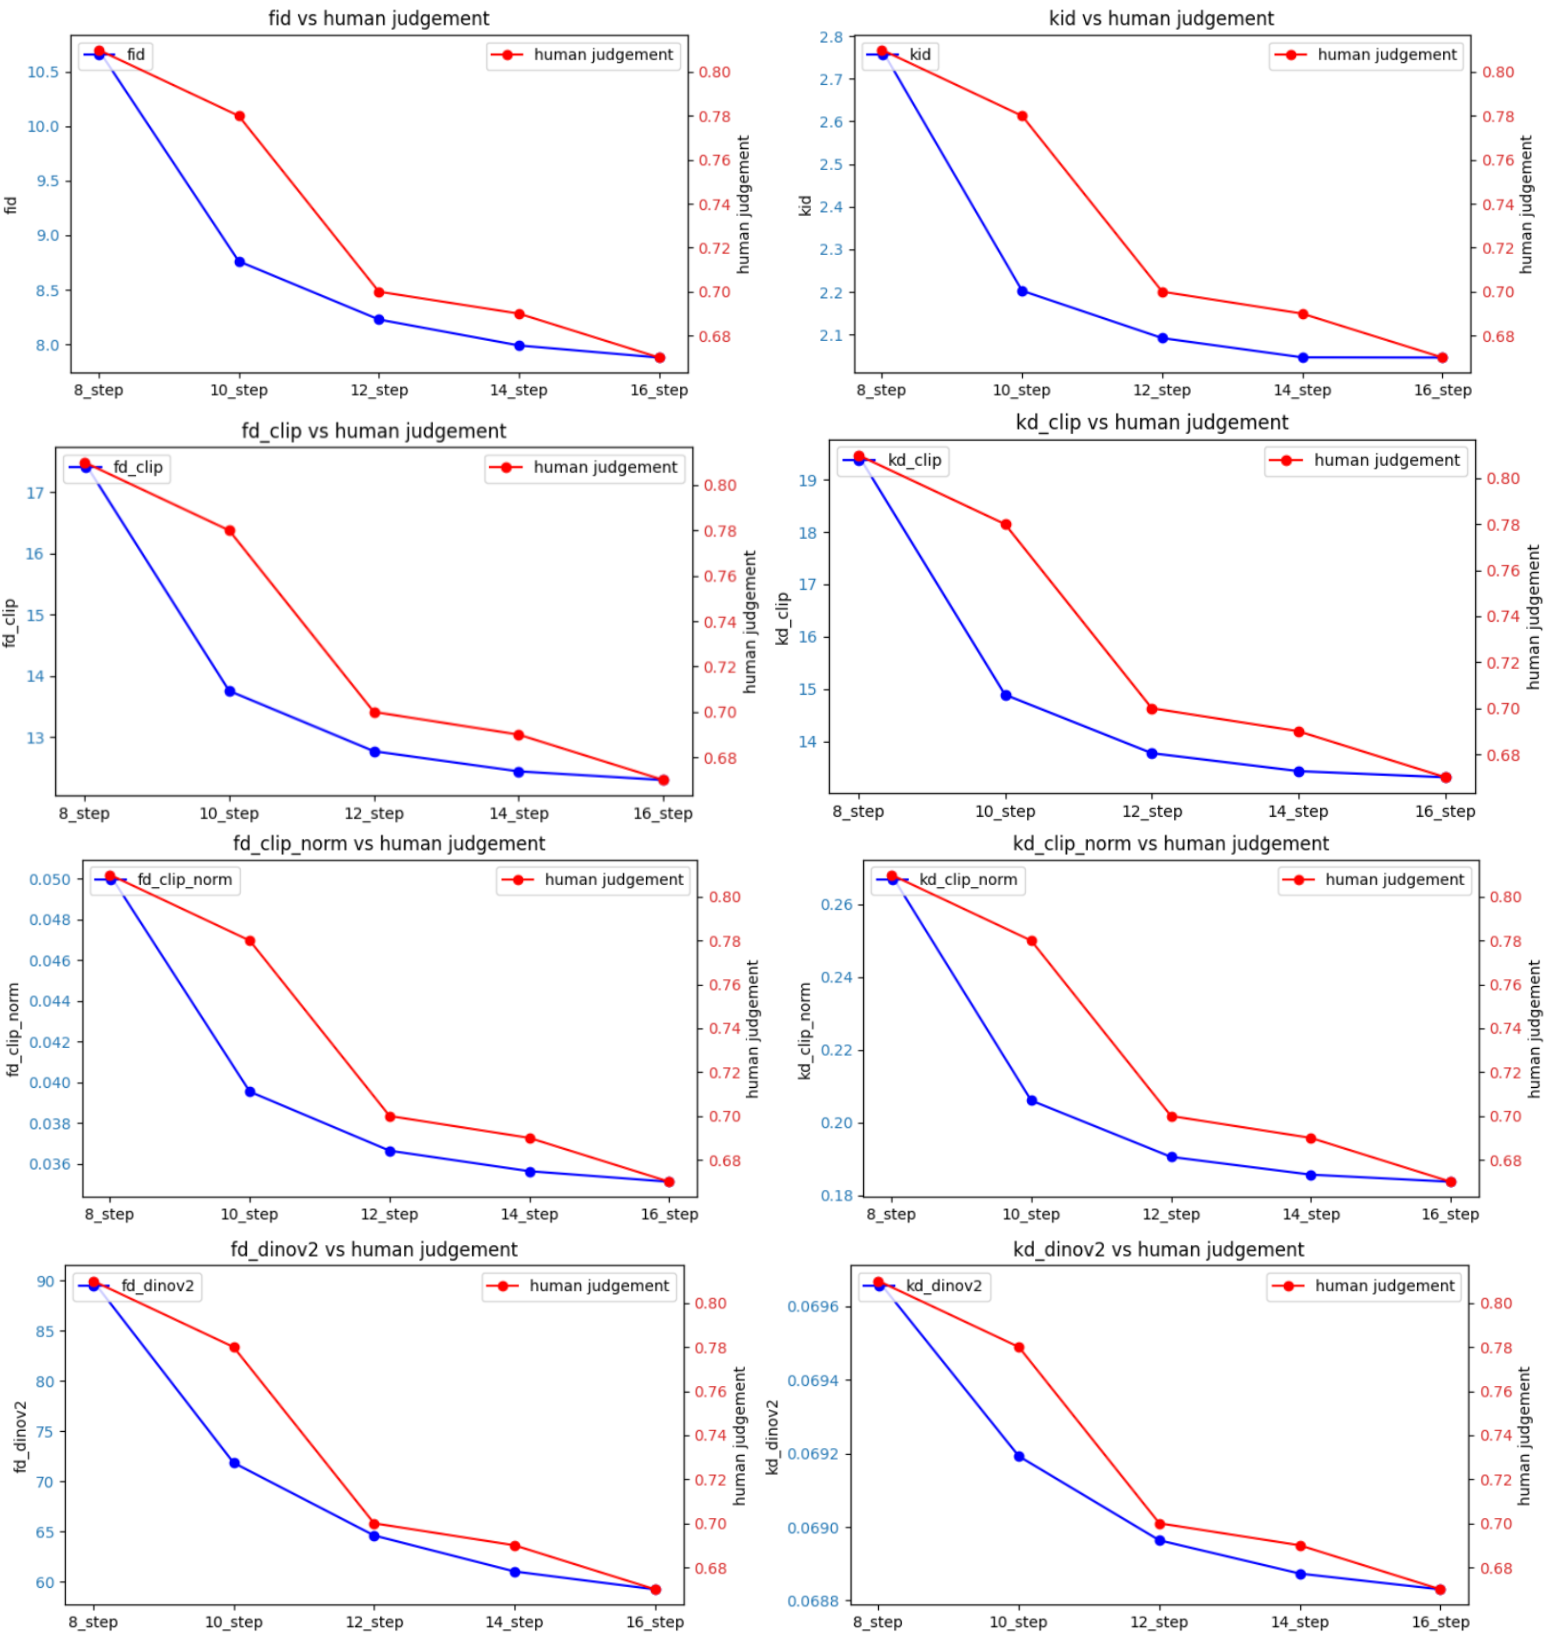
\includegraphics[width=16cm, height=17cm]{figs/mjhq30k_gen_steps.png}
\caption{Distance metrics measured on MJHQ30K dataset on models with different number of de-noising(generation) steps. The axes are the same on the Figure\ref{fig:coco_gen_steps}.}
\label{fig:mjhq30k_gen_steps}
\end{figure}

\subsubsection{Summary}
At the end of this experiment I can say that the FD\_DINOv2 metric performed the best. FID also showed excellent results. KID, FD\_CLIP, KD\_CLIP, FD\_CLIP\_norm and KD\_CLIP\_norm show poor results which may doubt CLIP as feature extractor. KD\_DINOv2 showed excellent results on the MJHQ30k dataset, but the exact opposite on COCO.

In this experiment, my assumption that KD\_DINOv2 shows correlation between generated images and MJHQ30k dataset and does not show with COCO because the model generates more contrasty and aesthetic images was confirmed.

After two experiments, I decided to remove metrics from CLIP as feature extractor since they show the worst results.

\subsection{Corrupted images by overlaying black squares on the images}
The third experiment I did was to corrupt the images that the model generated. I added black squares to the generated images and intuitively expected that the metric should show that the performance of the model was degraded. The idea for the experiment was taken from the original FID metric paper\cite{FID}.


It is important to note that I added black squares exactly on the generation items in the image. For example, if the prompt was “squirrel sitting on a tree”, then I put the square exactly on the part of the squirrel, not on the background of the image. At the Figure \ref{fig:images_with_black_squares} I show images generated images with black squares.

\begin{figure}[]
\centering
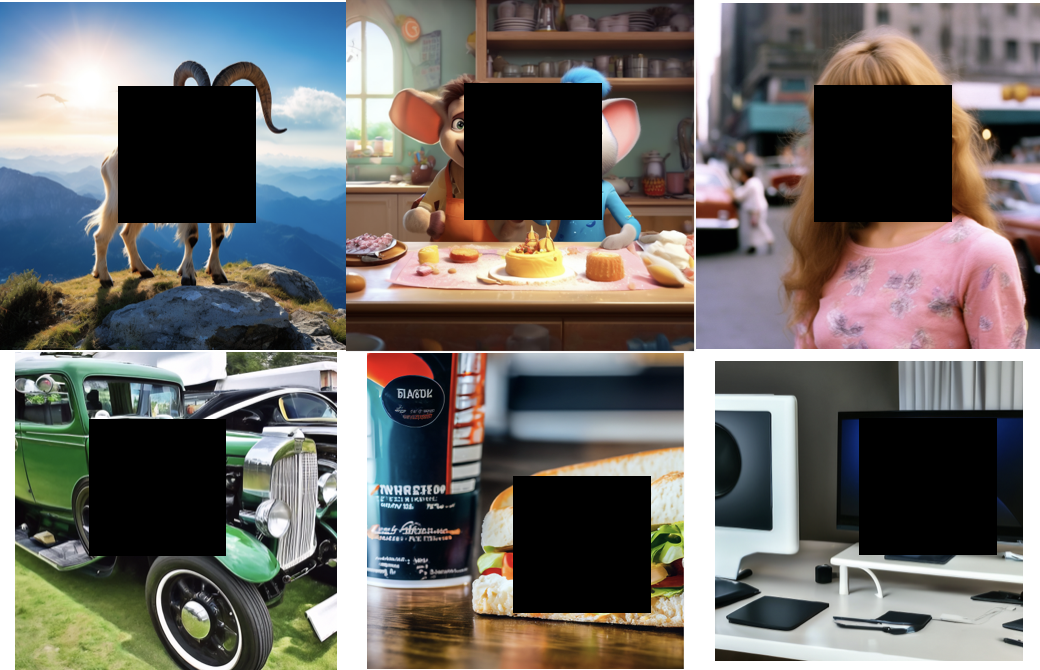
\includegraphics[width=7cm, height=6cm]{figs/images_with_black_squares.png}
\caption{Generated images with black squares.}
\label{fig:images_with_black_squares}
\end{figure}

\subsubsection{Summary}
As a result of the experiment, all metrics showed that pictures with painted black squares are worse, that is, less similar to the pictures from the dataset. Therefore, no additional information can be extracted from the experiment, because all metrics have performed perfectly.

\subsection{COS\_DINOv2 metric}
Separately, I conducted experiments for the COS\_DINOv2 metric, which I described in the “Methodology” chapter. I conducted two experiments: different numbers of de-noising steps and training steps. I used two datasets: COCO and MJHQ30k.

In all four experiments, the metric performed admirably. It correlates with human judgment in all experiments.

\begin{figure}[]
\centering
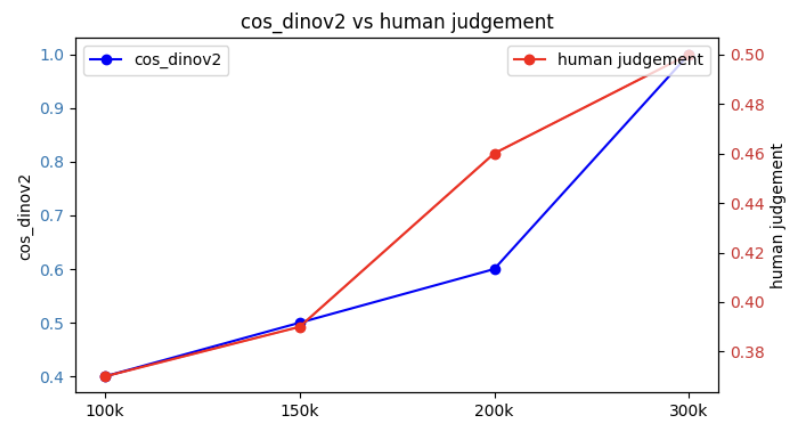
\includegraphics[width=9cm, height=5cm]{figs/coco_train_steps_COS_DINOv2.png}
\caption{COS\_DINOv2 on COCO dataset with different number of train steps. On the X-axis from left to right there are models with different number of steps from smaller to larger, i.e. from 100 thousand to 300 thousand. The left Y-axis shows the results of the metric, so the blue graph corresponds to the left Y-axis. On the right Y-axis are the results of human evaluation - this is the proportion of victories of the current model with the current number of training steps against the fully trained model (i.e. the model with 300 training steps). The red graph corresponds to the right Y-axis.}
\label{fig:coco_train_steps_cos_dinov2}
\end{figure}

\begin{figure}[]
\centering
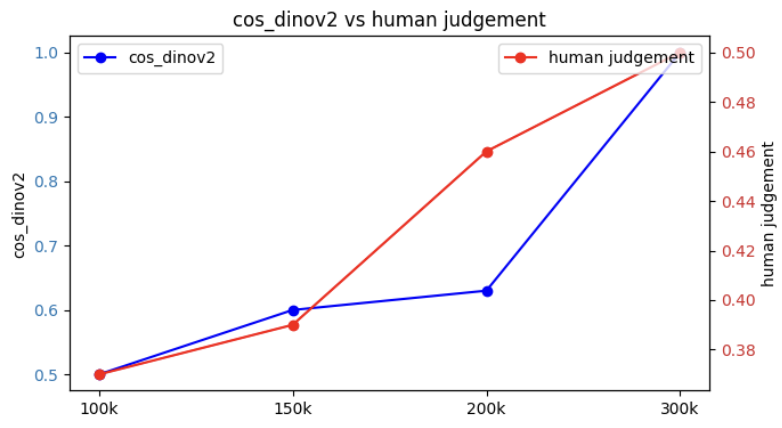
\includegraphics[width=9cm, height=5cm]{figs/mjhq30k_train_steps_COS_DINOv2.png}
\caption{COS\_DINOv2 on MJHQ30k dataset with different number of train steps. The axes are the same on the Figure \ref{fig:coco_train_steps_cos_dinov2}.}
\label{fig:mjhq30k_train_steps_cos_dinov2}
\end{figure}

\begin{figure}[]
\centering
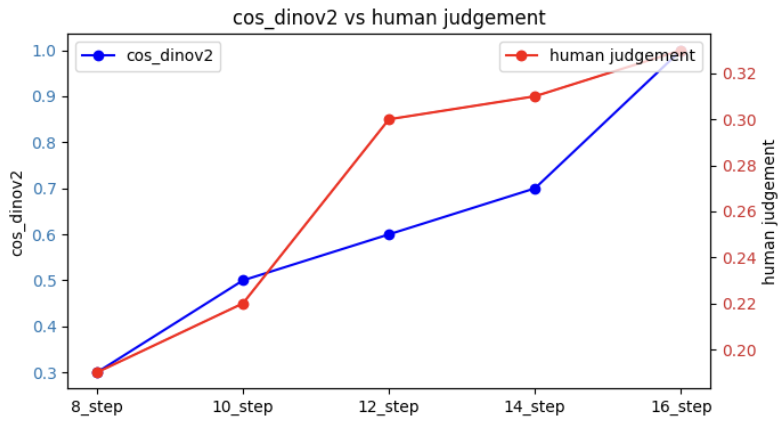
\includegraphics[width=9cm, height=5cm]{figs/coco_gen_steps_COS_DINOv2.png}
\caption{COS\_DINOv2 on COCO dataset with different number of de-noising steps. On the X-axis from left to right there are models with different number of steps from smaller to larger, i.e. from 8 steps to 16 steps. The left Y-axis shows the results of the metric, so the blue graph corresponds to the left Y-axis. On the right side of the Y-axis are the human evaluation results, which is the proportion of wins in the current model with the current number of de-noising steps against the 16-step model. The red graph corresponds to the right Y-axis.}
\label{fig:coco_gen_steps_cos_dinov2}
\end{figure}

\begin{figure}[]
\centering
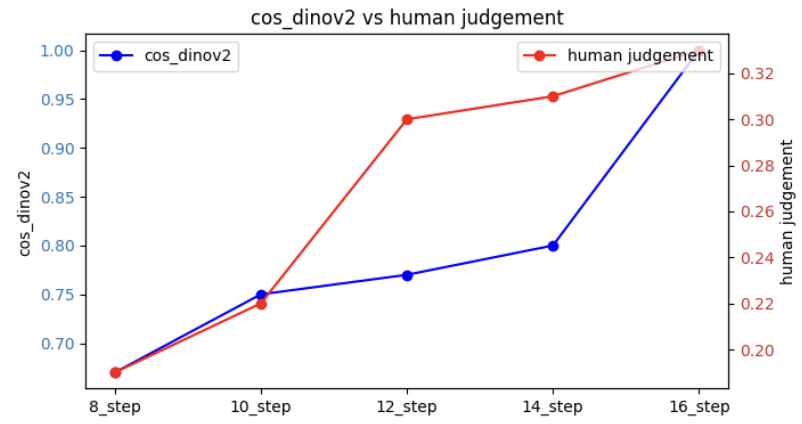
\includegraphics[width=9cm, height=5cm]{figs/mjhq30k_gen_steps_COS_DINOv2.png}
\caption{COS\_DINOv2 on MJHQ30k dataset with different number of de-noising steps. The axes are the same on the Figure \ref{fig:coco_gen_steps_cos_dinov2}.}
\label{fig:mjhq30k_gen_steps_cos_dinov2}
\end{figure}

\subsection{Summary for experiments with distance metrics}
From all the experiments performed, two metrics can be highlighted: FD\_DINOv2 and COS\_DINOv2. These are the metrics that show a precise correlation with human opinion in all experiments.

\section{Experiments with score metrics}
With scoring metrics, I did one experiment. It was to train Imagen with different number of steps and see how the metrics would behave. I use four metrics in total: CLIPScore\cite{CLIPScore}, CLIPSCore with MCLIP, ImageReward\cite{Image_reward}, HPSv2\cite{HPSv2} .I use the same models I used in the distance metrics experiments. I used the prompts from the COCO dataset. The resulting graphs of the experiment are shown in Figure \ref{fig:coco_train_steps_score_metrics}.

\begin{figure}[]
\centering
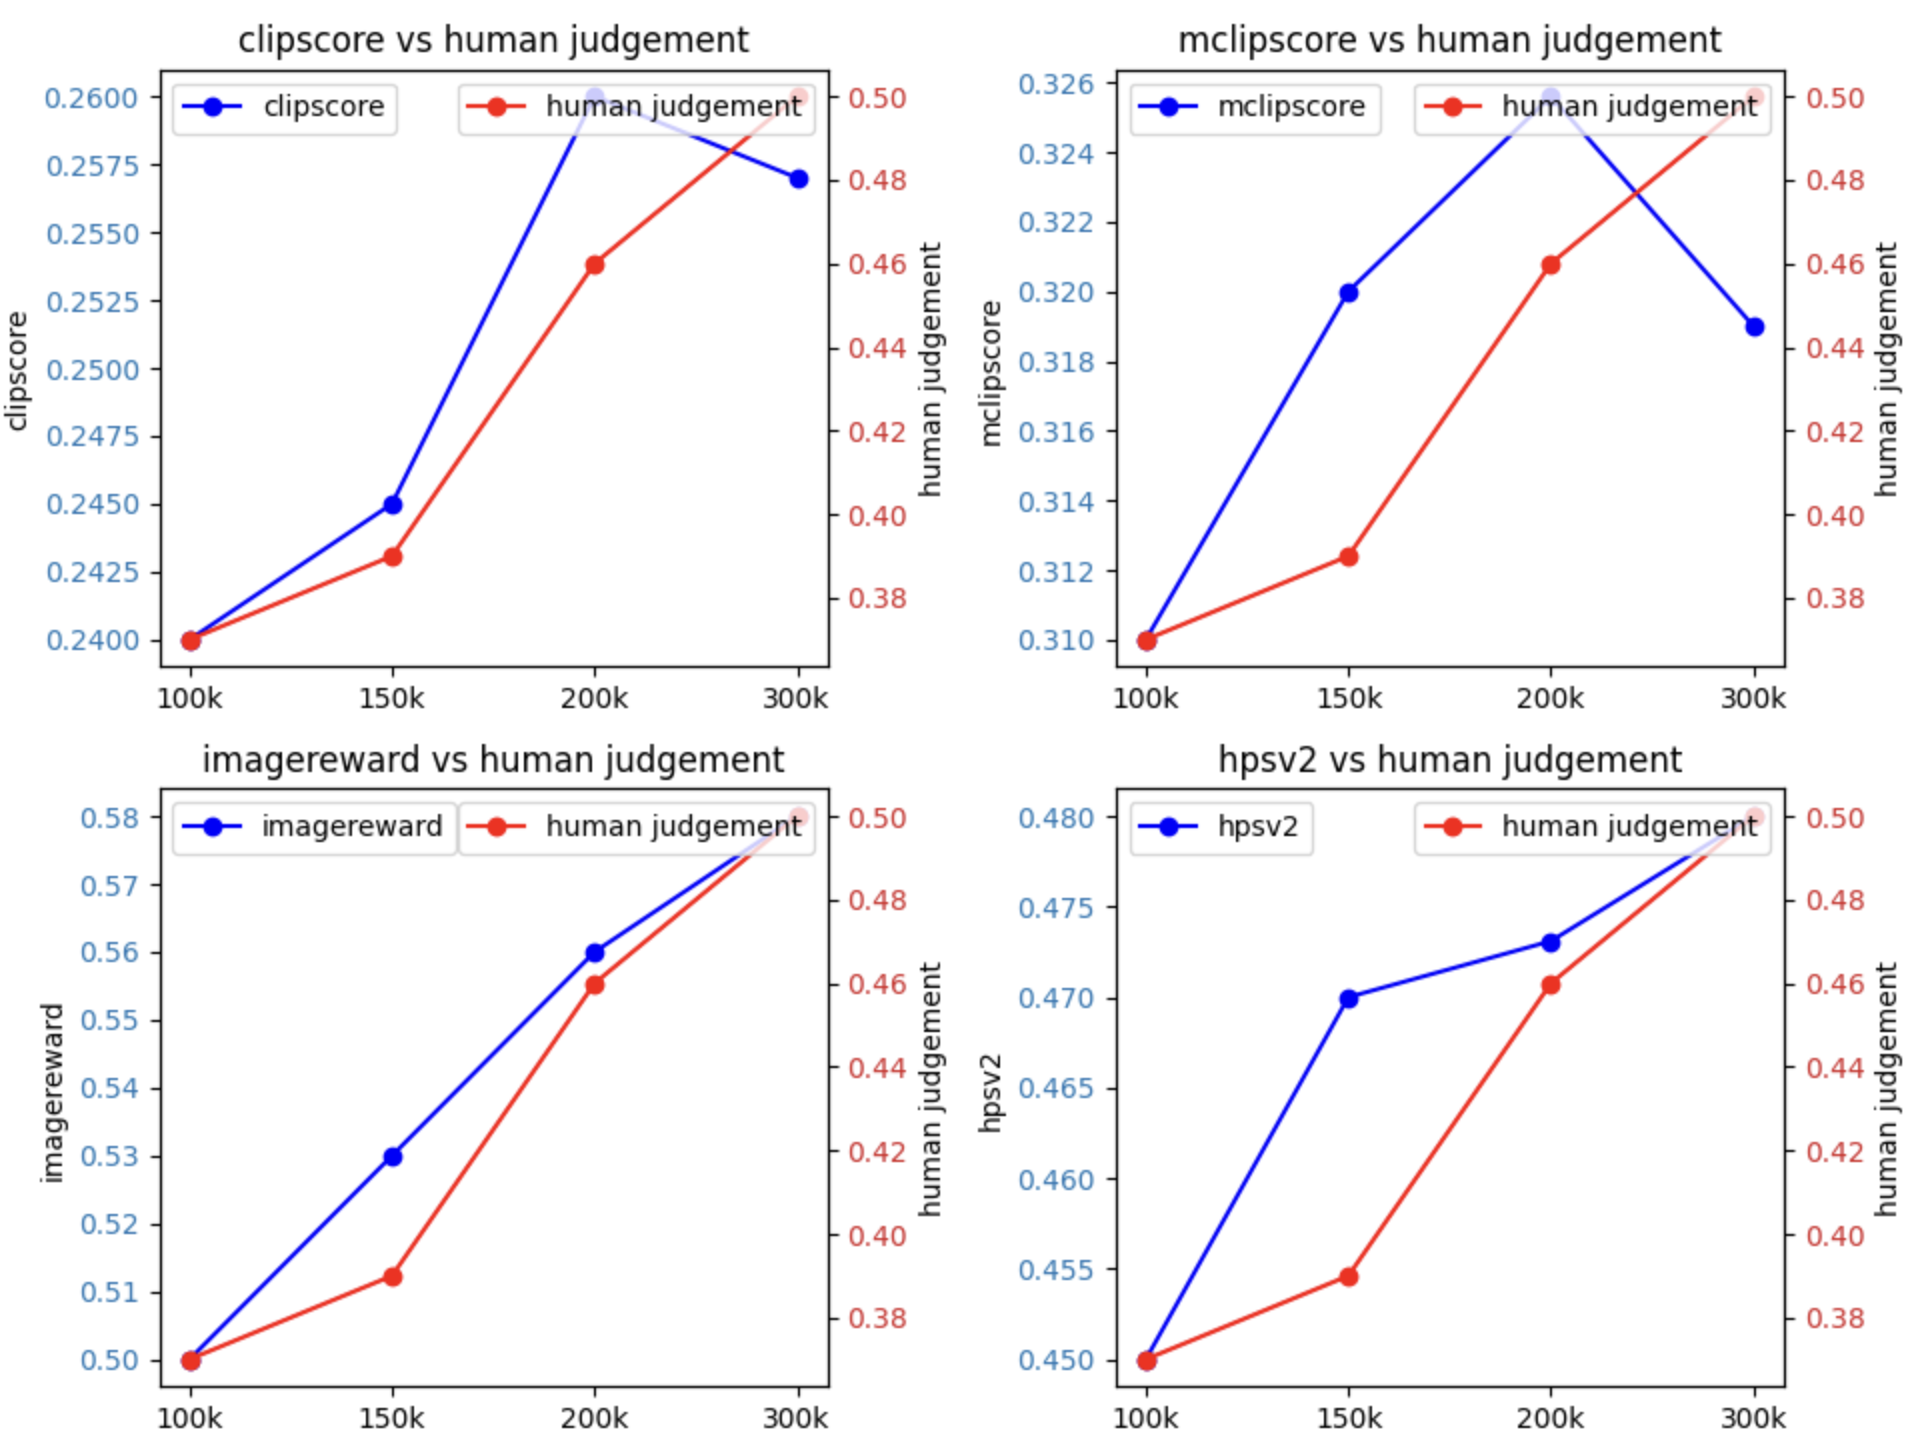
\includegraphics[width=15cm, height=9cm]{figs/coco_train_steps_score_metrics.png}
\caption{Score metrics on COCO dataset with different number of train steps. The axes are the same on the Figure \ref{fig:coco_train_steps_cos_dinov2}.}
\label{fig:coco_train_steps_score_metrics}
\end{figure}

My experiment shows similarity of CLIPScore and CLIPScore metrics on MCLIP feature extractor, also it can be seen that ImageReward and HPSv2 correlate better with human judgement than CLIPScore and CLIPScore on MCLIP chips. ImageReward correlates best of all so it becomes the leader in score metrics.

\chapter{Discussion}
\label{chap:discussion}
In this chapter, I want to explain the usefulness of my research based on analyzing the amount of time and money saved by using offline metrics rather than using humans to determine the best text-to-image generation model. I will also describe what future research can be done.

\section{Research application}
Suppose we have two generative text-to-image models and we want to understand which one is better. Suppose we have two methods: human evaluation and offline metrics. Using offline metrics does not require a lot of time and does not require any money at all, so I will calculate the amount of time and money spent using the human evaluation method.


Suppose we have a dataset of 10000 prompts. Each model generates one image per prompt, so annotators need to make 10000 comparisons, but for better evaluation we need to use three annotators, so annotators get 30000 comparisons. To estimate which model is better I take the proportion of evaluations on a particular model which determines whether the model is better or worse. For example, if out of 30000 comparisons 21000 were for the first model, then the first model scores 0.7 and the second model scores 0.3.

Assuming that an annotator spends 6 seconds for one comparison, it would take three annotators to annotate 30000 binary comparisons: 10000 * 6 / 60 / 60 = 16.67 hours of continuous work by three people.

Since labor payment depends on many factors it is difficult to objectively estimate how much money can be spent on annotating such a dataset. I say that an annotator gets \$$x$ dollars for one binary comparison or \$$y$ dollars for one hour of work.

It turns out that in total it may take $16.67 * 3 * y=\$50y$ dollars to partition such a dataset if count payment in hours or \$$30000x$ dollars if paid for each binary comparison.

Assuming that the annotator gets one cent per three images marked, or \$4 per hour of work, it would cost \$200 dollars to mark up the dataset if we consider hourly rates or \$100 dollars if paid for each binary comparison. I take an average estimate of \$150 dollars.

And this is only to test one experiment, and if consider that there can be dozens of such experiments, let's say about 50 only for one research, then 150*50=\$7500 dollars can be spent to explore one research question.

Calculations show that a good offline metric saves \$7500 dollars and 2500 person-hours just to explore a single research question.

\section{Future works}
I can deduce three ways to further explore the issue of offline metrics.

The first way is to study what each metric is responsible for, i.e. what aspect of the image each metric considers more important. By aspects I mean aesthetics, defectiveness, and relevance to text. From my experiments I assume that distance metrics are related to aesthetics and score metrics to text relevance, but to verify my assumption I need to do some more experiments.

The second way is to study score metrics better, to conduct more experiments to identify a more clear leader between all score metrics.

The third way is to study offline metrics that change the generative model into a discriminative model. I took this approach from the SelfEval\cite{SelfEval} article and it seems very promising to me.
\chapter{Conclusion}
\label{chap:conclusion}
In this thesis, I analyzed existing offline metrics for evaluating text-to-image generative models. I identified standard metrics such as FID and CLIPScore, and found that two types of metrics can be defined: distance metrics and score metrics.

I experimented with FID and CLIPScore metrics. For the FID metric, I changed the feature extractor and the method of calculating the distance between the two distributions. I used three feature extractors: InceptionV3, CLIP and DINOv2. I also used two distance computing methods: fréchet distance and kernel distance. As a result, I got 6 metrics: FID\cite{FID}, KID, FD\_CLIP, KD\_CLIP\cite{KD_CLIP}, FD\_DINOv2\cite{FD_DINOv2} and KD\_DINOv2. I conducted experiments in which I determined the metric that correlates best with a human judgement is FD\_DINOv2.

For score metrics I changed feature extractor and dataset for finetuning. I ended up experimenting with several metrics: CLIPScore\cite{CLIPScore}, CLIPScore with MCLIP as feature extractor, ImageReward\cite{Image_reward} and HPSv2\cite{HPSv2}. As a result of the experiment I get that ImageReward correlates best with human judgement.

I also derived my unique COS\_DINOv2 metric. The distinctive specificity of the metric is that it takes into account that real images taken from dataset and generated images refer to the same prompts. My metric showed excellent correlation with human opinion on a level with FD\_DINOv2.


In conclusion, my work has made a huge step in the development of offline metrics for text-to-image generative models. I proposed to divide current metrics into two types: distance metrics and score metrics. I highlighted the best metrics of both kinds and proposed my own, new offline metrics. I hope that my research contributes to further development in the field of offline metrics for text-to-image generative models.

%% REFERENCES
\printbibliography[ =bibintoc,title={Bibliography cited}]
\end{document}